\documentclass[conference]{IEEEtran}
\usepackage[utf8]{inputenc}
\usepackage[T1]{fontenc}
\usepackage[spanish]{babel}
\usepackage{amsmath,amssymb}
\usepackage{graphicx}
\usepackage{caption}
\usepackage{float}
\usepackage{listings}
\lstset{
  basicstyle=\ttfamily\small,
  columns=fullflexible,
  breaklines=true,
  postbreak=\mbox{\textcolor{red}{$\hookrightarrow$}\space},
  extendedchars=true,
  literate={á}{{\'a}}1 {é}{{\'e}}1 {í}{{\'i}}1 {ó}{{\'o}}1 {ú}{{\'u}}1 {ñ}{{\~n}}1 {Á}{{\'A}}1 {É}{{\'E}}1 {Í}{{\'I}}1 {Ó}{{\'O}}1 {Ú}{{\'U}}1 {Ñ}{{\~N}}1
}
\usepackage{xcolor}
\usepackage{booktabs}
\usepackage{hyperref}

\title{Tarea 02: Implementación Manual de Regresión Lineal con Descenso de Gradiente}

\author{
Jose Miguel Gonzalez Barrantes\\
Carné: 2023087564\\
Emmanuel Rodríguez\\
Carné: 2023146102\\
Escuela de Ingeniería en Computación\\
Instituto Tecnológico de Costa Rica\\
Profesor: Steven Andrey Pacheco Portugués\\
Curso: IC6200 Inteligencia Artificial\\
Fecha: Martes 24 de marzo de 2026
}

\setlength{\parskip}{6pt}
\setlength{\parindent}{0pt}
\renewcommand{\baselinestretch}{1.05}

\lstset{
  basicstyle=\ttfamily\small,
  keywordstyle=\color{blue}\bfseries,
  commentstyle=\color{gray},
  stringstyle=\color{teal},
  numbers=left,
  numberstyle=\tiny,
  frame=single,
  breaklines=true,
  showstringspaces=false,
  captionpos=b,
  xleftmargin=6pt,
  xrightmargin=6pt
}

\newcommand{\CodeBlockSpaceBefore}{\vspace{8pt}}
\newcommand{\CodeBlockSpaceAfter}{\vspace{10pt}}

\begin{document}
\maketitle

\begin{abstract}
En este trabajo se implementó un modelo de regresión lineal desde cero utilizando únicamente NumPy y Pandas, aplicándolo al dataset \textit{Student Performance Prediction}. Primero se realizó una exploración del conjunto de datos mediante estadísticas descriptivas y visualizaciones como histogramas, diagramas de caja, diagramas de dispersión y una matriz de correlación. Después, el dataset se dividió manualmente en entrenamiento, validación y prueba. Finalmente, se implementaron dos variantes de descenso del gradiente, Batch Gradient Descent y Mini-Batch Gradient Descent, y se evaluó su desempeño mediante el error cuadrático medio (MSE), comparando sus resultados y analizando su convergencia. Además de la ejecución de distintas pruebas con datos para así analizar de mejor manera su funcionamiento.
\end{abstract}

\section{Introducción}

La regresión lineal es uno de los modelos más básicos y útiles dentro del aprendizaje automático supervisado. Su objetivo es modelar la relación que existe entre un conjunto de variables predictoras y una variable objetivo continua. Aunque existen librerías que permiten entrenar este tipo de modelos con pocas líneas de código, en esta tarea se optó por una implementación manual.

El propósito principal fue implementar una regresión lineal con descenso del gradiente usando únicamente NumPy, evitando librerías de \textit{machine learning} como \texttt{scikit-learn}. Esto permitió trabajar directamente con elementos fundamentales como son el cálculo del gradiente, la actualización de parámetros y la evaluación del modelo en entrenamiento, validación y prueba.

Además de la implementación del modelo, se realizó un análisis exploratorio de datos con el fin de entender mejor la estructura del conjunto de datos, detectar posibles valores atípicos y observar qué variables presentaban una relación más clara con la variable objetivo. Esto fue importante porque permitió justificar posteriormente el uso de un modelo de regresión lineal, especialmente al evidenciar la hipótesis de que algunas relaciones eran aproximadamente lineales.

\section{Descripción del dataset}

Se trabajó con el conjunto de datos \textit{Student Performance Prediction}, el cual contiene aproximadamente 10\,000 registros sintéticos de estudiantes. Cada fila representa un estudiante y cada columna corresponde a una característica asociada a su desempeño académico, es decir una variable de estudio.

Las variables presentes son las siguientes:

\begin{itemize}
    \item \textbf{Hours Studied}: horas dedicadas al estudio.
    \item \textbf{Previous Scores}: calificaciones previas.
    \item \textbf{Extracurricular Activities}: participación en actividades extracurriculares.
    \item \textbf{Sleep Hours}: horas de sueño.
    \item \textbf{Sample Question Papers Practiced}: cantidad de prácticas realizadas.
    \item \textbf{Performance Index}: índice de rendimiento académico, utilizado como variable objetivo.
\end{itemize}

La variable objetivo del problema fue \texttt{Performance Index}, mientras que el resto de variables se utilizaron como entradas del modelo.

Según el repositorio donde se descargó, el dataset es sintético, lo cual ayuda a explicar por qué presenta distribuciones bastante limpias, poca presencia de ruido y relaciones relativamente claras entre ciertas variables. Aun así, resulta útil para practicar el flujo completo de lectura, análisis, modelado y evaluación.

\section{Lectura y exploración del dataset}

Se utilizó Pandas para cargar el archivo CSV en un \textit{DataFrame} y explorar su estructura general, incluyendo filas, columnas, tipos de variables y estadísticas descriptivas. Adicionalmente para poder trabajar con los datos de manera mucho más ordenada.

\subsection{Carga del dataset}

A continuación se presenta un segmento de código el cual fue utilizado para poder cargar el dataset en el dataframe:

\CodeBlockSpaceBefore
\begin{lstlisting}[language=Python, caption={Carga inicial del dataset}]
import pandas as pd
import numpy as np

df = pd.read_csv("student_performance.csv")
df.head()
\end{lstlisting}
\CodeBlockSpaceAfter

\subsection{Tipos de variables}

Las variables \texttt{Hours Studied}, \texttt{Previous Scores}, \texttt{Sleep Hours} y \texttt{Sample Question Papers Practiced} fueron de tipo entero, mientras que \texttt{Performance Index} fue un float. Por otro lado, \texttt{Extracurricular Activities} correspondió a una variable categórica con valores como \texttt{Yes} y \texttt{No}.

Se menciona este aspecto debido a que fue importante porque la variable categórica no podía utilizarse directamente en el modelo, por lo que tiempo después fue necesario transformarla a valores numéricos. Además, la identificación de tipos de variables facilitó la selección de visualizaciones para poder hacer el análisis que se pidió.

\subsection{Estadísticas descriptivas}

Se calcularon media, desviación estándar, mínimos y máximos de las variables numéricas. Los resultados obtenidos indican que el dataset presenta una distribución razonable y sin comportamientos extremos. Los valores exactos se pueden consultar al momento de correr el Notebook.

\CodeBlockSpaceBefore
\begin{lstlisting}[language=Python, caption={Cálculo de estadísticas descriptivas}]
print("Media:")
print(df.mean(numeric_only=True))

print("\nDesviación estándar:")
print(df.std(numeric_only=True))

print("\nMínimos:")
print(df.min(numeric_only=True))

print("\nMáximos:")
print(df.max(numeric_only=True))
\end{lstlisting}
\CodeBlockSpaceAfter

En general, la variable \texttt{Performance Index} presentó un rango amplio entre 10 y 100, lo que sugiere una diversidad muy alta en el rendimiento académico de los estudiantes. De manera similar, \texttt{Previous Scores} mostró una diferencia notable, lo cual resultó fuerte influencia sobre la variable objetivo en análisis posteriores.

La media de \texttt{Hours Studied} indicó que, en promedio, los estudiantes dedican una cantidad moderada de tiempo al estudio. Igualmente \texttt{Sleep Hours} mostró una media relativamente estable, lo que sugiere que los hábitos de sueño no varían de manera extrema entre las observaciones que se hicieron. En cuanto a \texttt{Sample Question Papers Practiced}, sus valores también se distribuyeron dentro de un rango acotado, sin la presencia de extremos fuera de lo común.

\section{Análisis exploratorio de datos}

\subsection{Histogramas}

Los histogramas permitieron observar la distribución de las variables numéricas del dataset. En la mayoría de los casos se encontró una distribución relativamente uniforme, especialmente en \texttt{Hours Studied}, \texttt{Previous Scores}, \texttt{Sleep Hours} y \texttt{Sample Question Papers Practiced}. Además, la variable \texttt{Performance Index} mostró una forma más cercana a una distribución aproximadamente normal (campana), concentrándose en valores intermedios y en los extremos con cantidad menores de datos.

\begin{figure}[H]
    \centering
    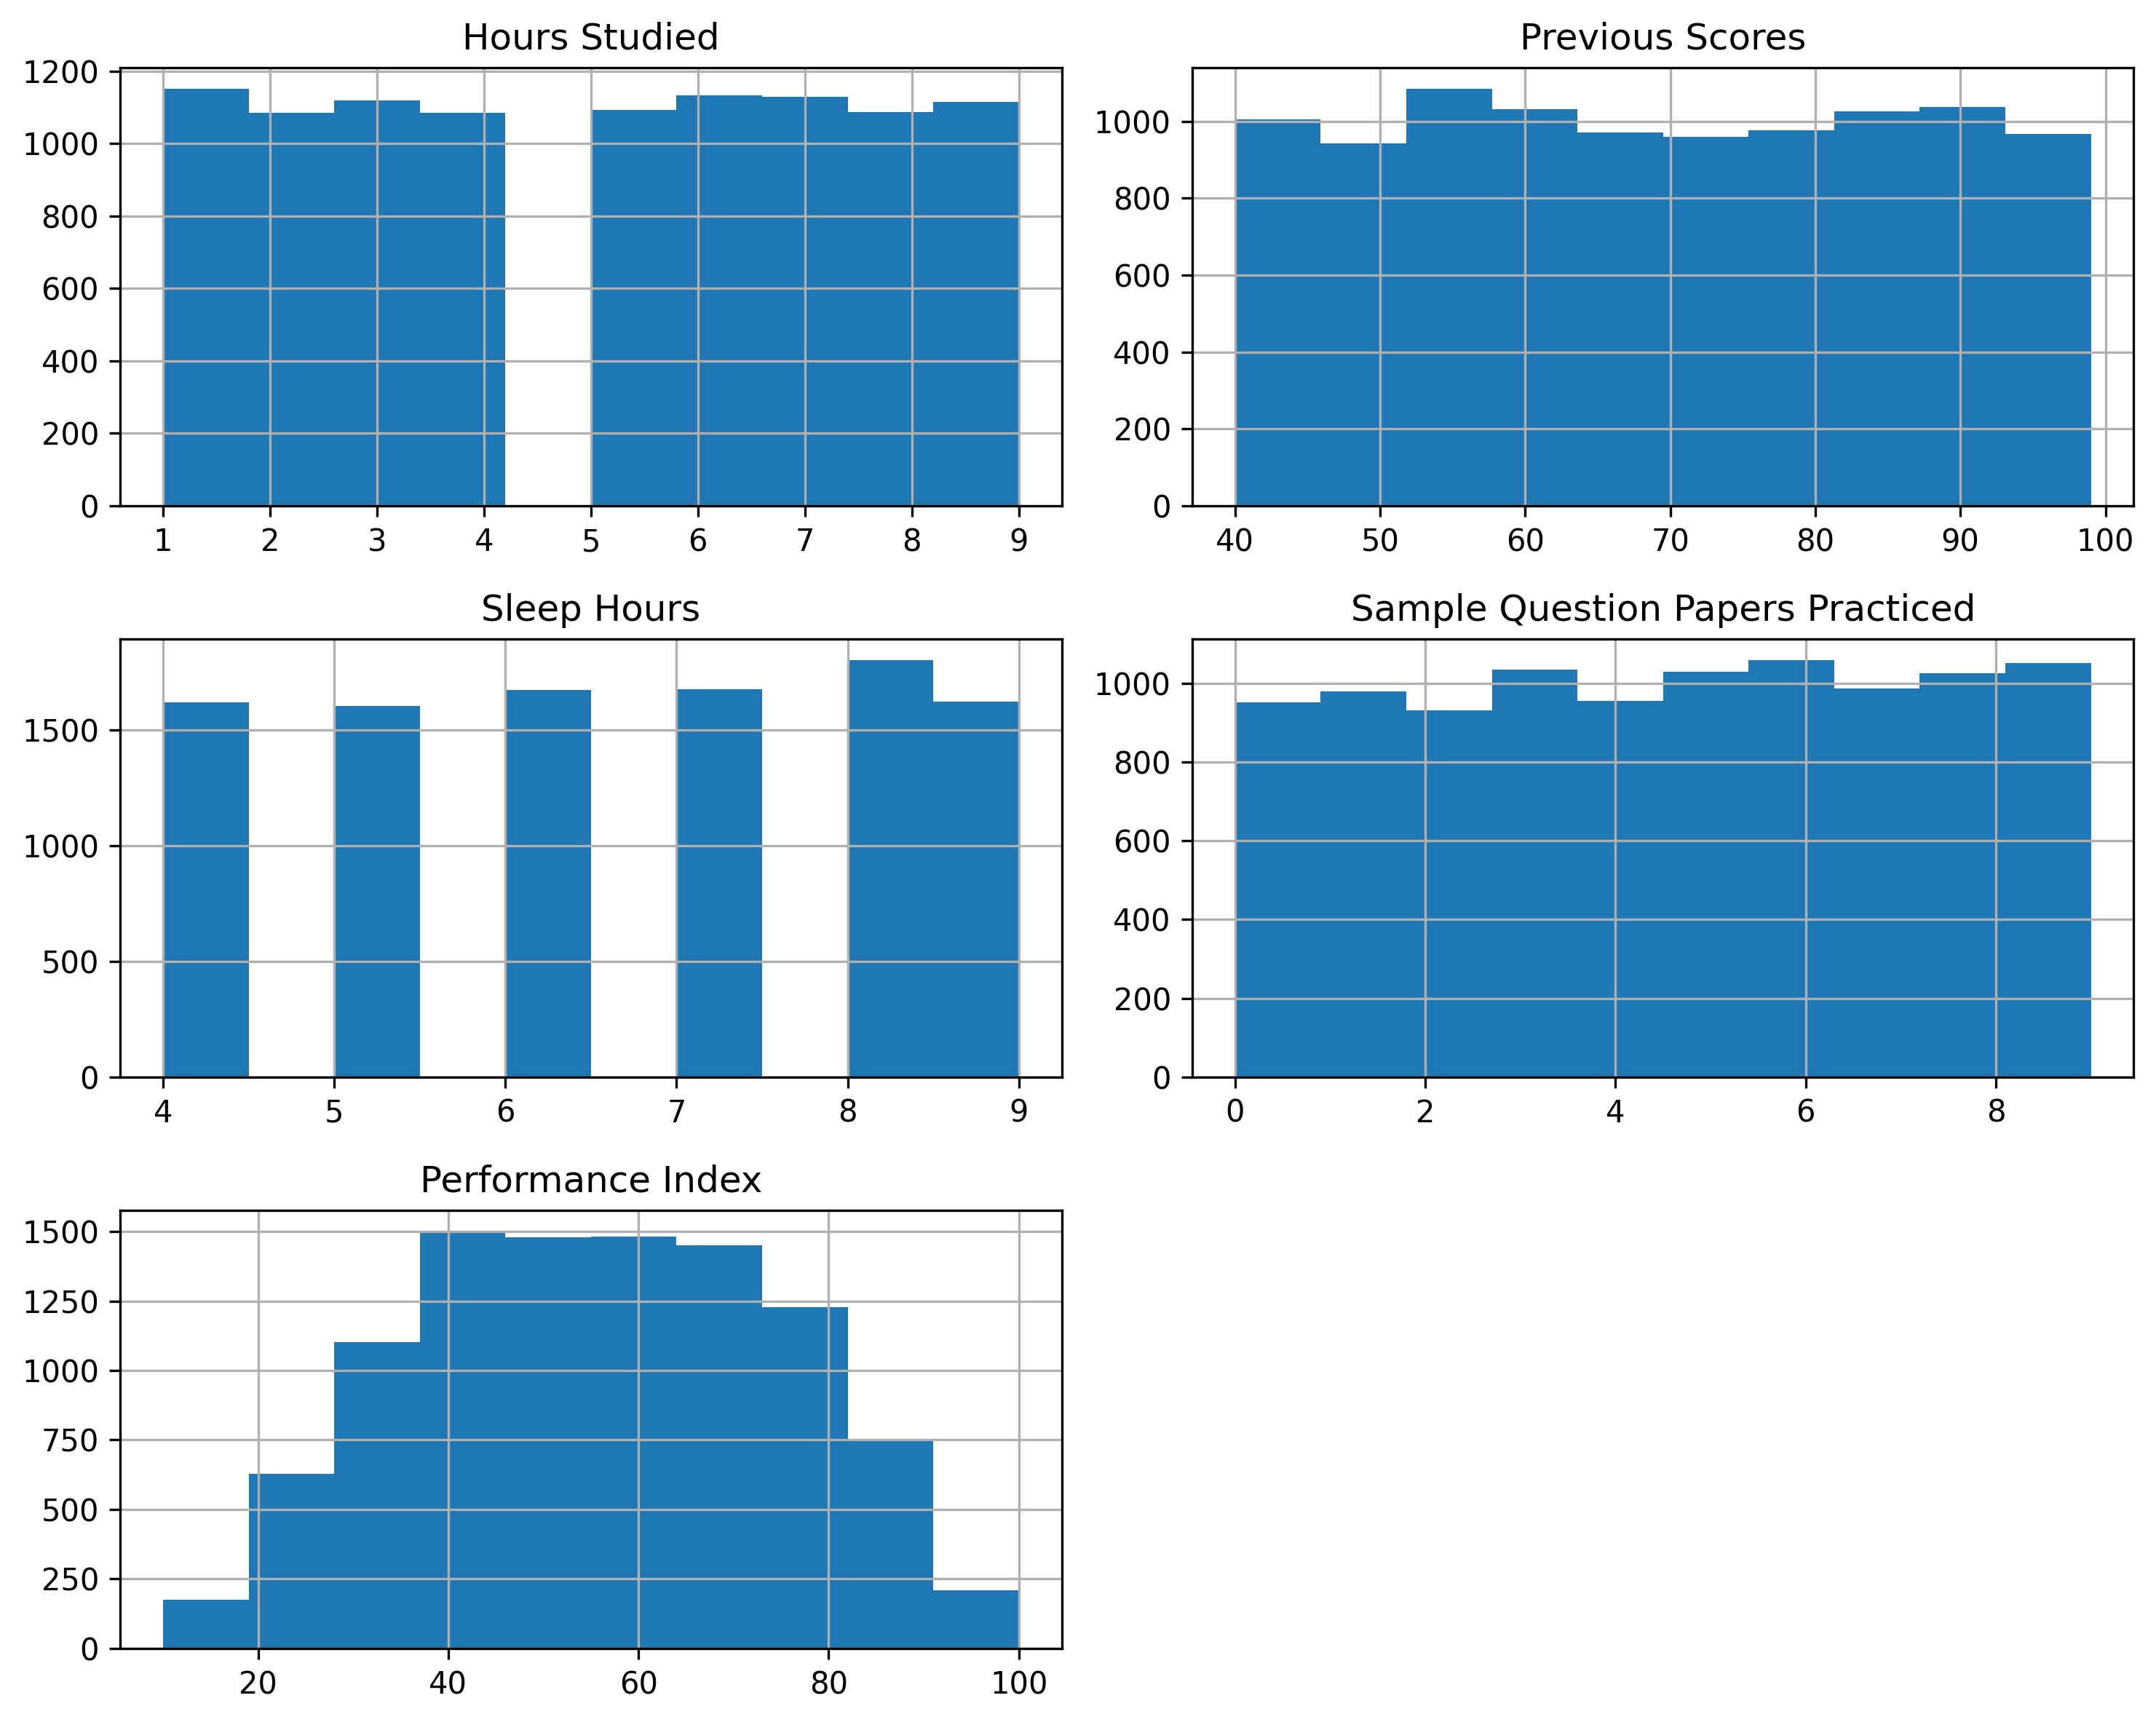
\includegraphics[width=0.48\textwidth]{histogramas.png}
    \caption{Histogramas de las variables numéricas del dataset.}
\end{figure}

Un aspecto importante observado en algunos histogramas fue la presencia de pequeños huecos o separaciones entre barras. Esto no se vió como un problema en los datos o la forma que se estaban procesando, sino como una consecuencia de que varias variables son discretas y toman únicamente valores enteros. Por lo que cuando se intenta agrupar estos datos en intervalos, algunos espacios visuales quedan vacíos, lo cual es completamente normal.

Los histogramas también permitieron notar que el \texttt{Performance Index} no se concentra únicamente en valores altos o bajos, sino que cubre un rango amplio con mayor densidad en la zona media.

\subsection{Diagramas de caja}

Los diagramas de caja se utilizaron para detectar posibles valores atípicos. A partir de la visualización no se observaron valores fuera de los rangos esperados, por lo que no se evidenciaron datos sobresalientes significativos. Esto indicó que el dataset era consistente y no requería un tratamiento adicional para outliers. A continuación se presenta el diagrama de cajas realizado, no obstante en el Notebook se incluya una con los puntos negros y con el uso de colores para así tener un mejor análisis.

\begin{figure}[H]
    \centering
    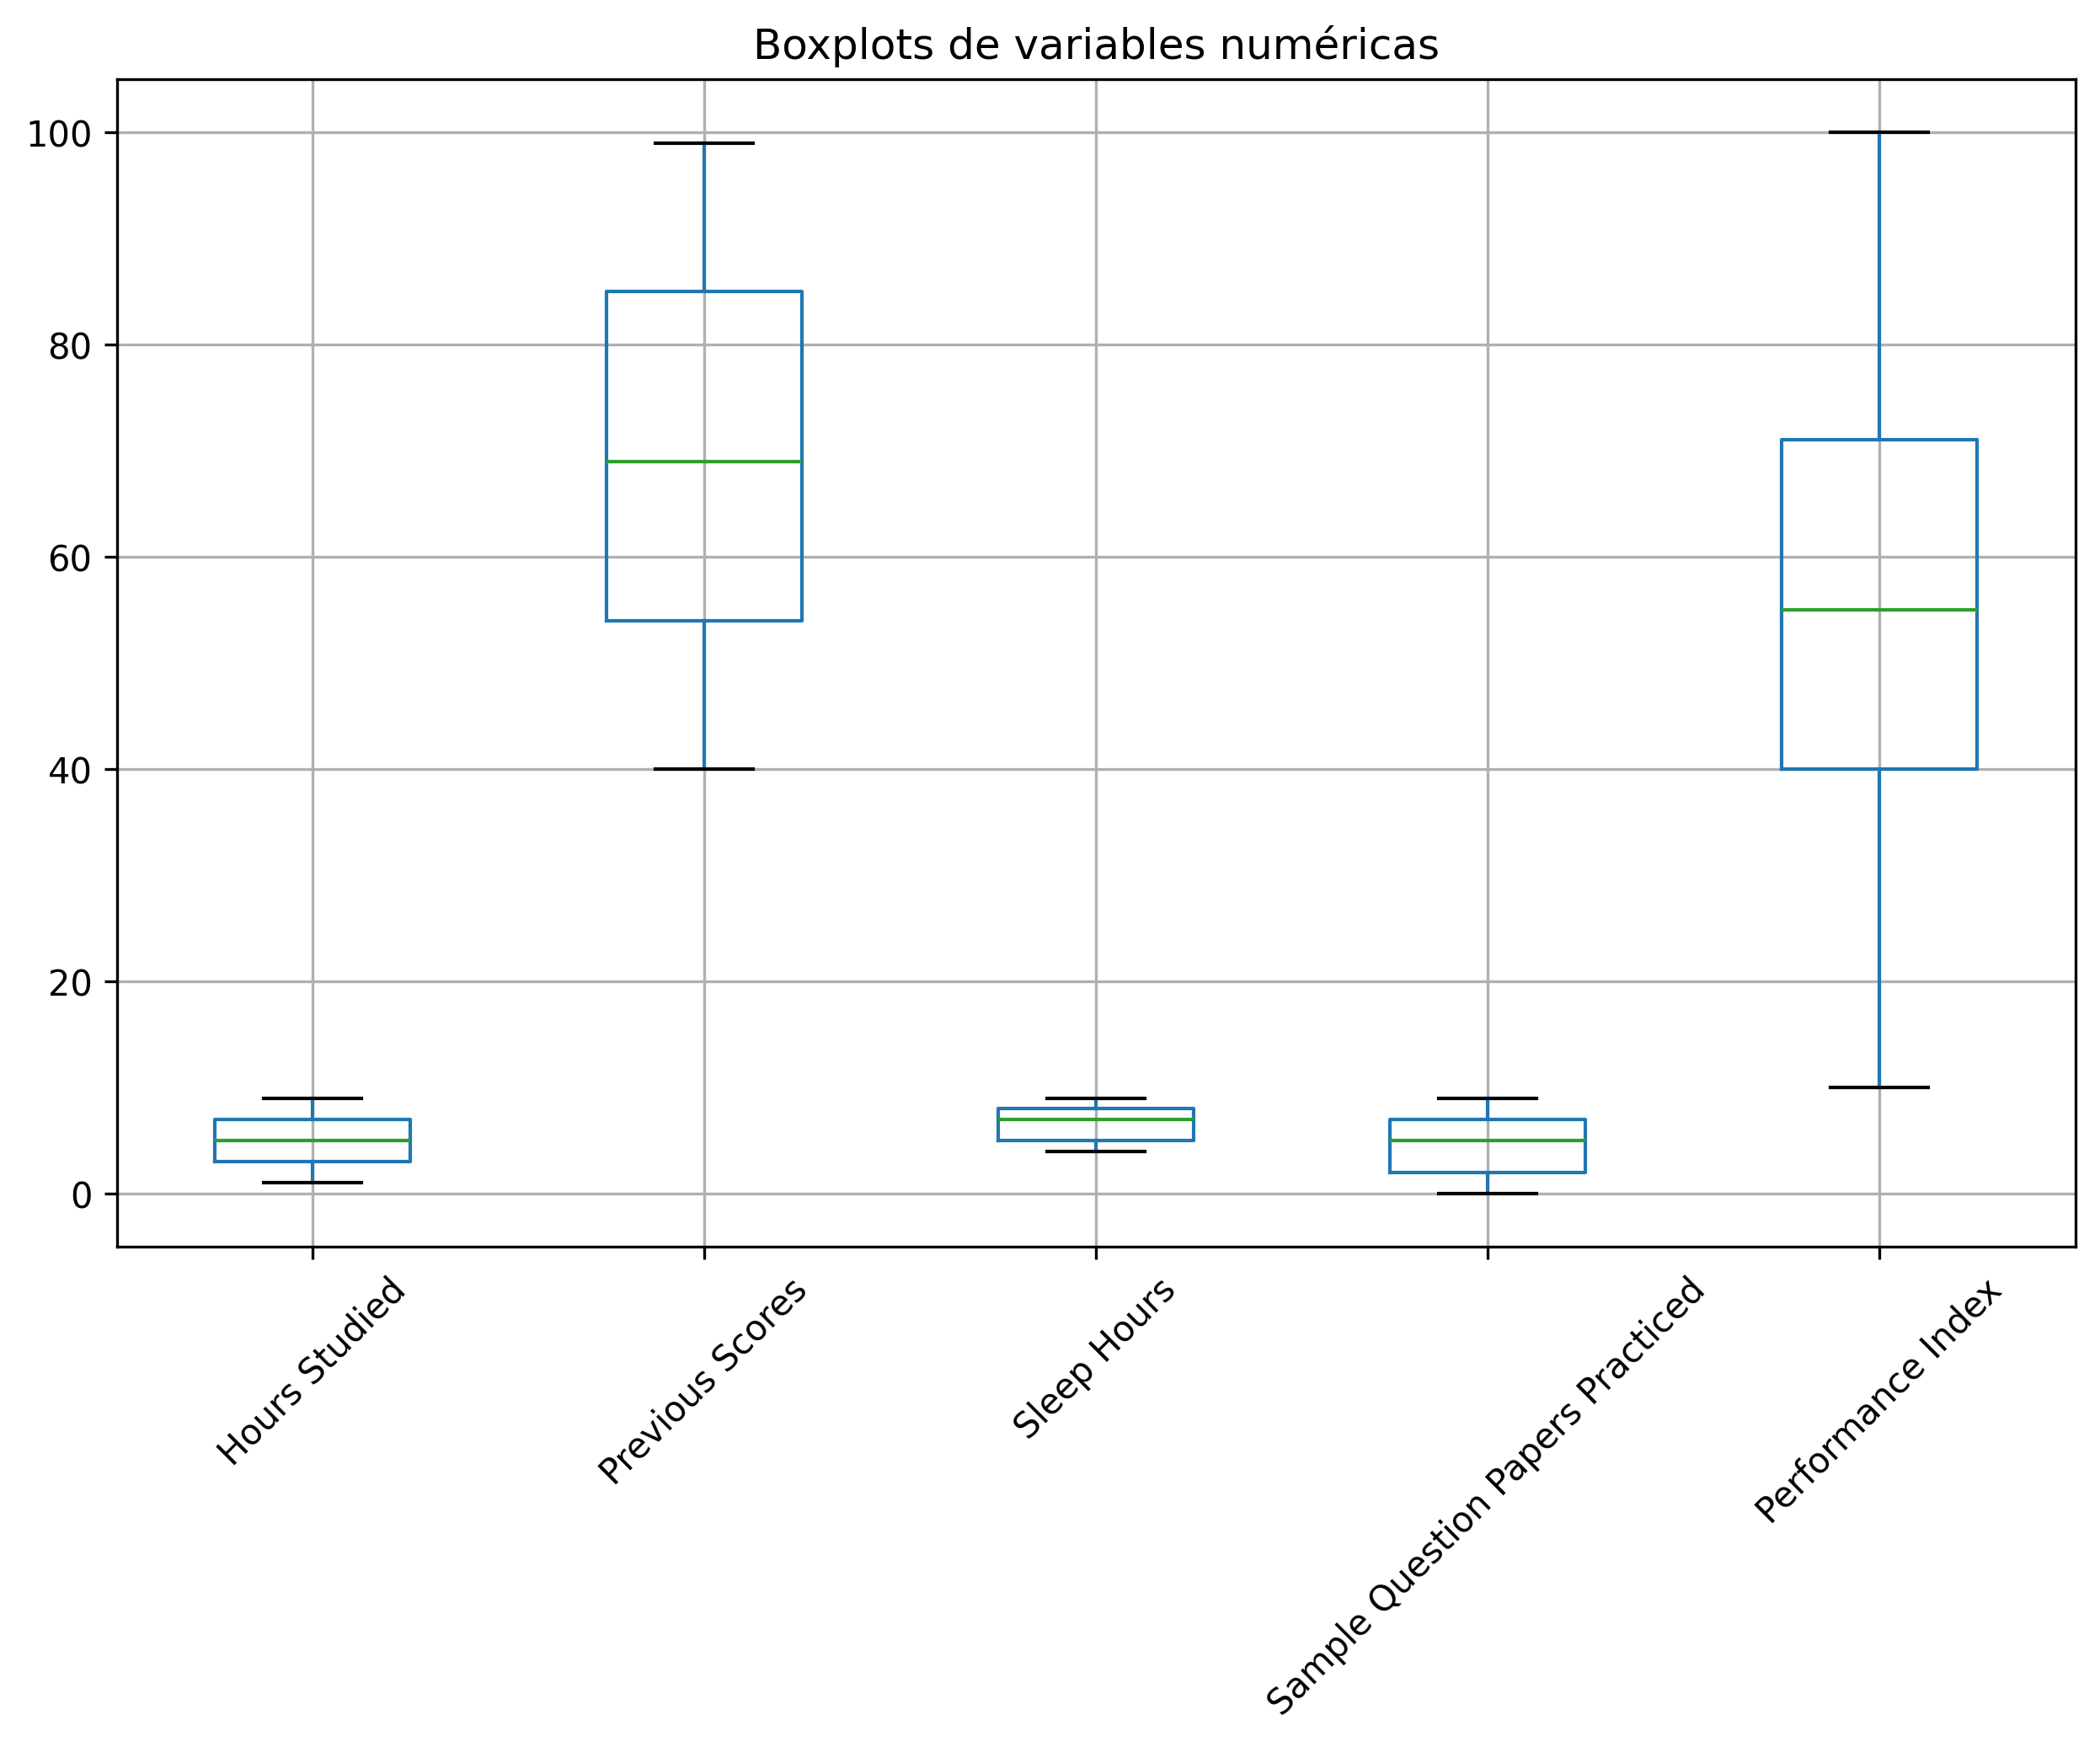
\includegraphics[width=0.48\textwidth]{boxplots.png}
    \caption{Diagramas de caja para las variables numéricas.}
\end{figure}

En los boxplots se observó que variables como \texttt{Previous Scores} y \texttt{Performance Index} presentaron una dispersión mayor en comparación con \texttt{Hours Studied}, \texttt{Sleep Hours} y \texttt{Sample Question Papers Practiced}. Esto tiene sentido porque tanto las calificaciones previas como el rendimiento académico tienden a variar más entre estudiantes.

La ausencia de valores fuera de los bigotes fue especialmente importante, ya que permitió concluir que no había evidencia visual de outliers relevantes. Esto simplificó el proceso de modelado que se haría más adelante, pues no fue necesario eliminar observaciones ni aplicar tratamientos especiales para valores extremos.

\subsection{Diagramas de dispersión}

Se analizaron las relaciones entre cada característica y la variable objetivo. En estos gráficos, cada punto representa una observación del dataset, donde el eje horizontal corresponde a una característica y el eje vertical al \texttt{Performance Index}. Este tipo de visualización fue especialmente útil para identificar tendencias lineales y posibles patrones de asociación.

\subsubsection{Hours Studied vs Performance Index}

\begin{figure}[H]
    \centering
    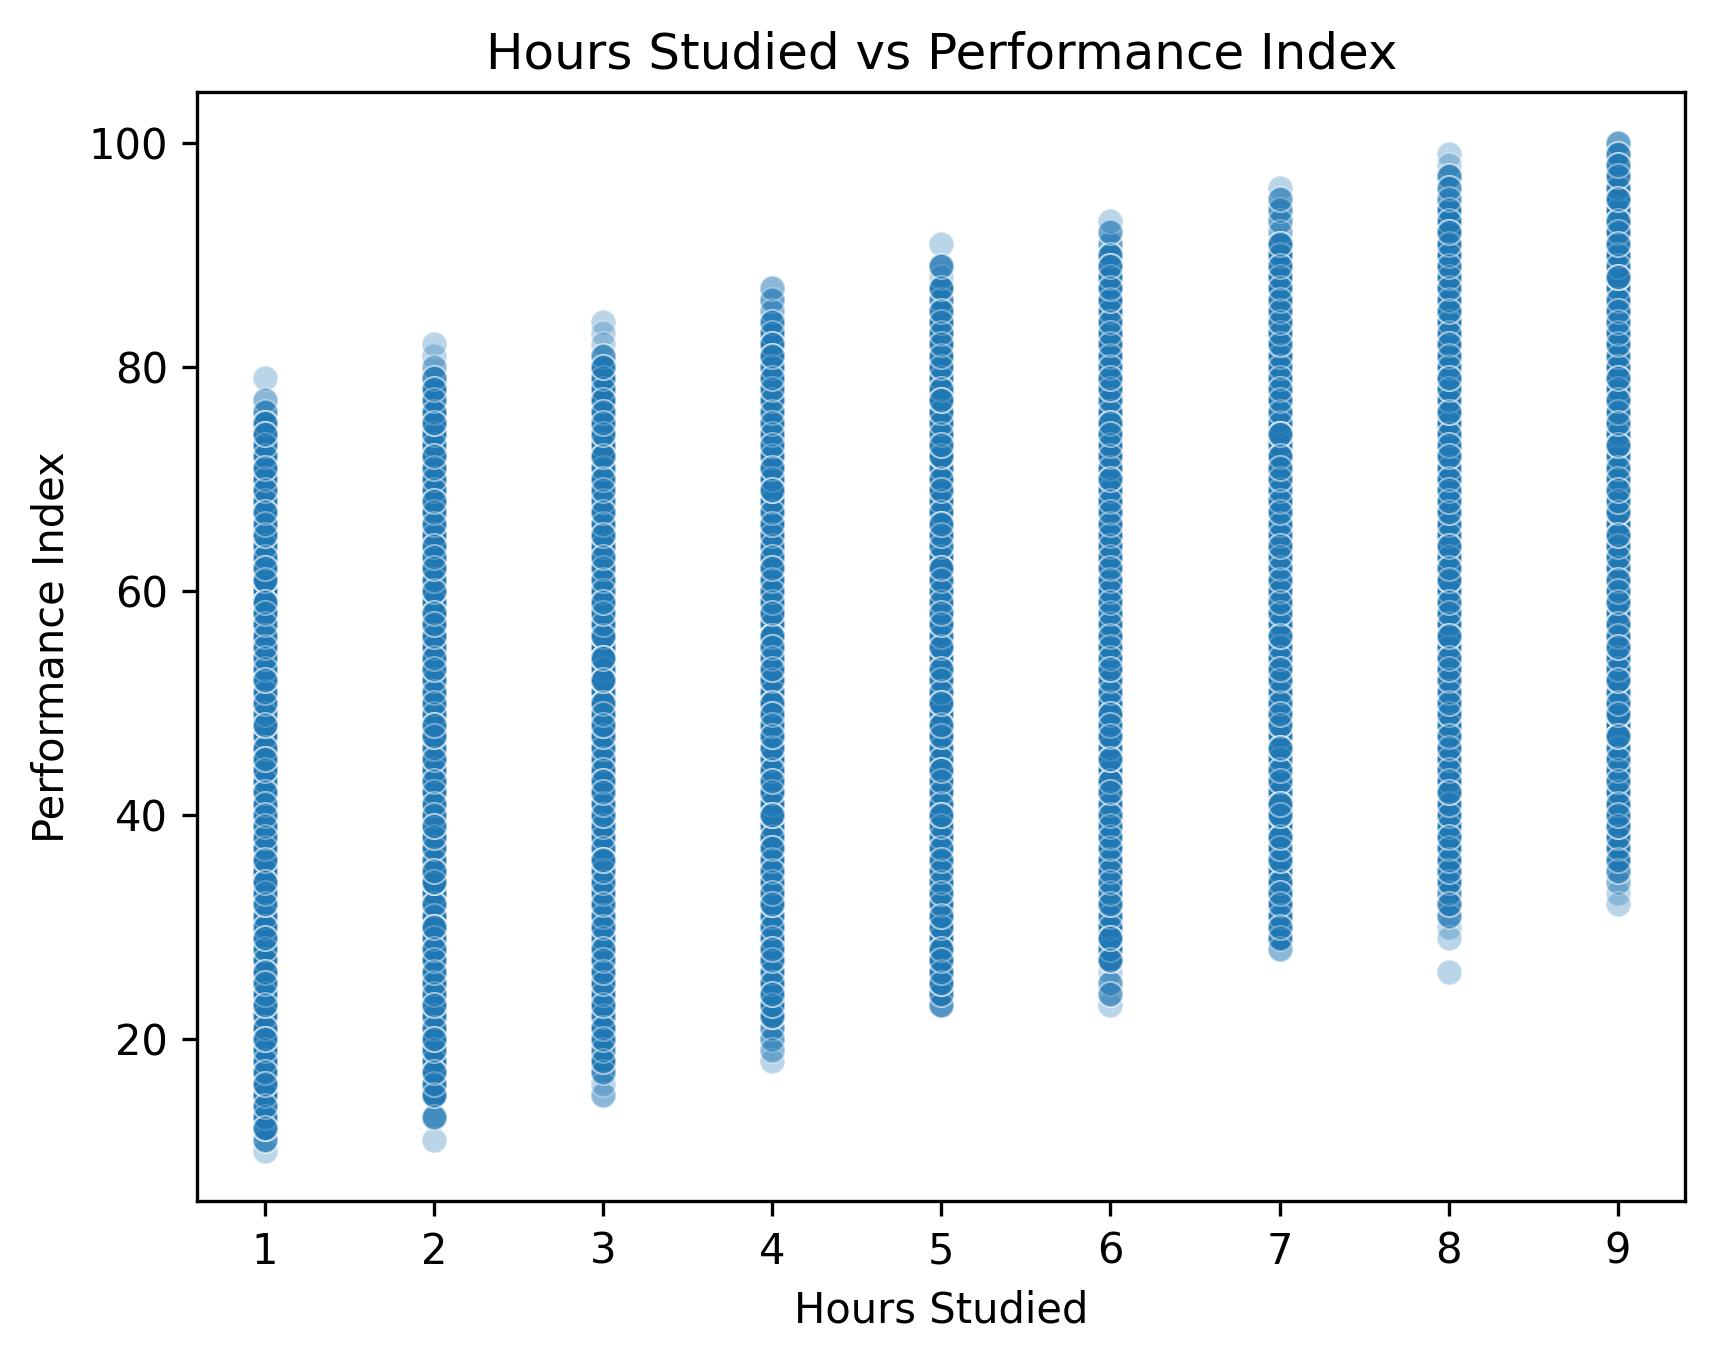
\includegraphics[width=0.44\textwidth]{hours_studied.png}
    \caption{Relación entre Hours Studied y Performance Index.}
\end{figure}

En este gráfico se observó una relación positiva entre las horas de estudio y el rendimiento académico. Aunque la dispersión fue mayor que en otras variables, sí se aprecia una tendencia ascendente, esto debido a que se puede ver que, conforme aumentan las horas estudiadas, también tiende a incrementarse el \texttt{Performance Index}. Con este evento podermos dar la idea de qque el tiempo dedicado al estudio influye de manera moderada sobre el desempeño, lo cual tiene sentido.

A como se vió anteriormente en algunos otros diagrams, las líneas verticales observadas en este gráfico no corresponden a un error, sino al hecho de que \texttt{Hours Studied} es una variable discreta que solo toma ciertos valores enteros. Por lo tanto, muchas observaciones comparten el mismo valor en el eje horizontal y se agrupan verticalmente, dando ese efecto de linea "recta".

\subsubsection{Previous Scores vs Performance Index}

\begin{figure}[H]
    \centering
    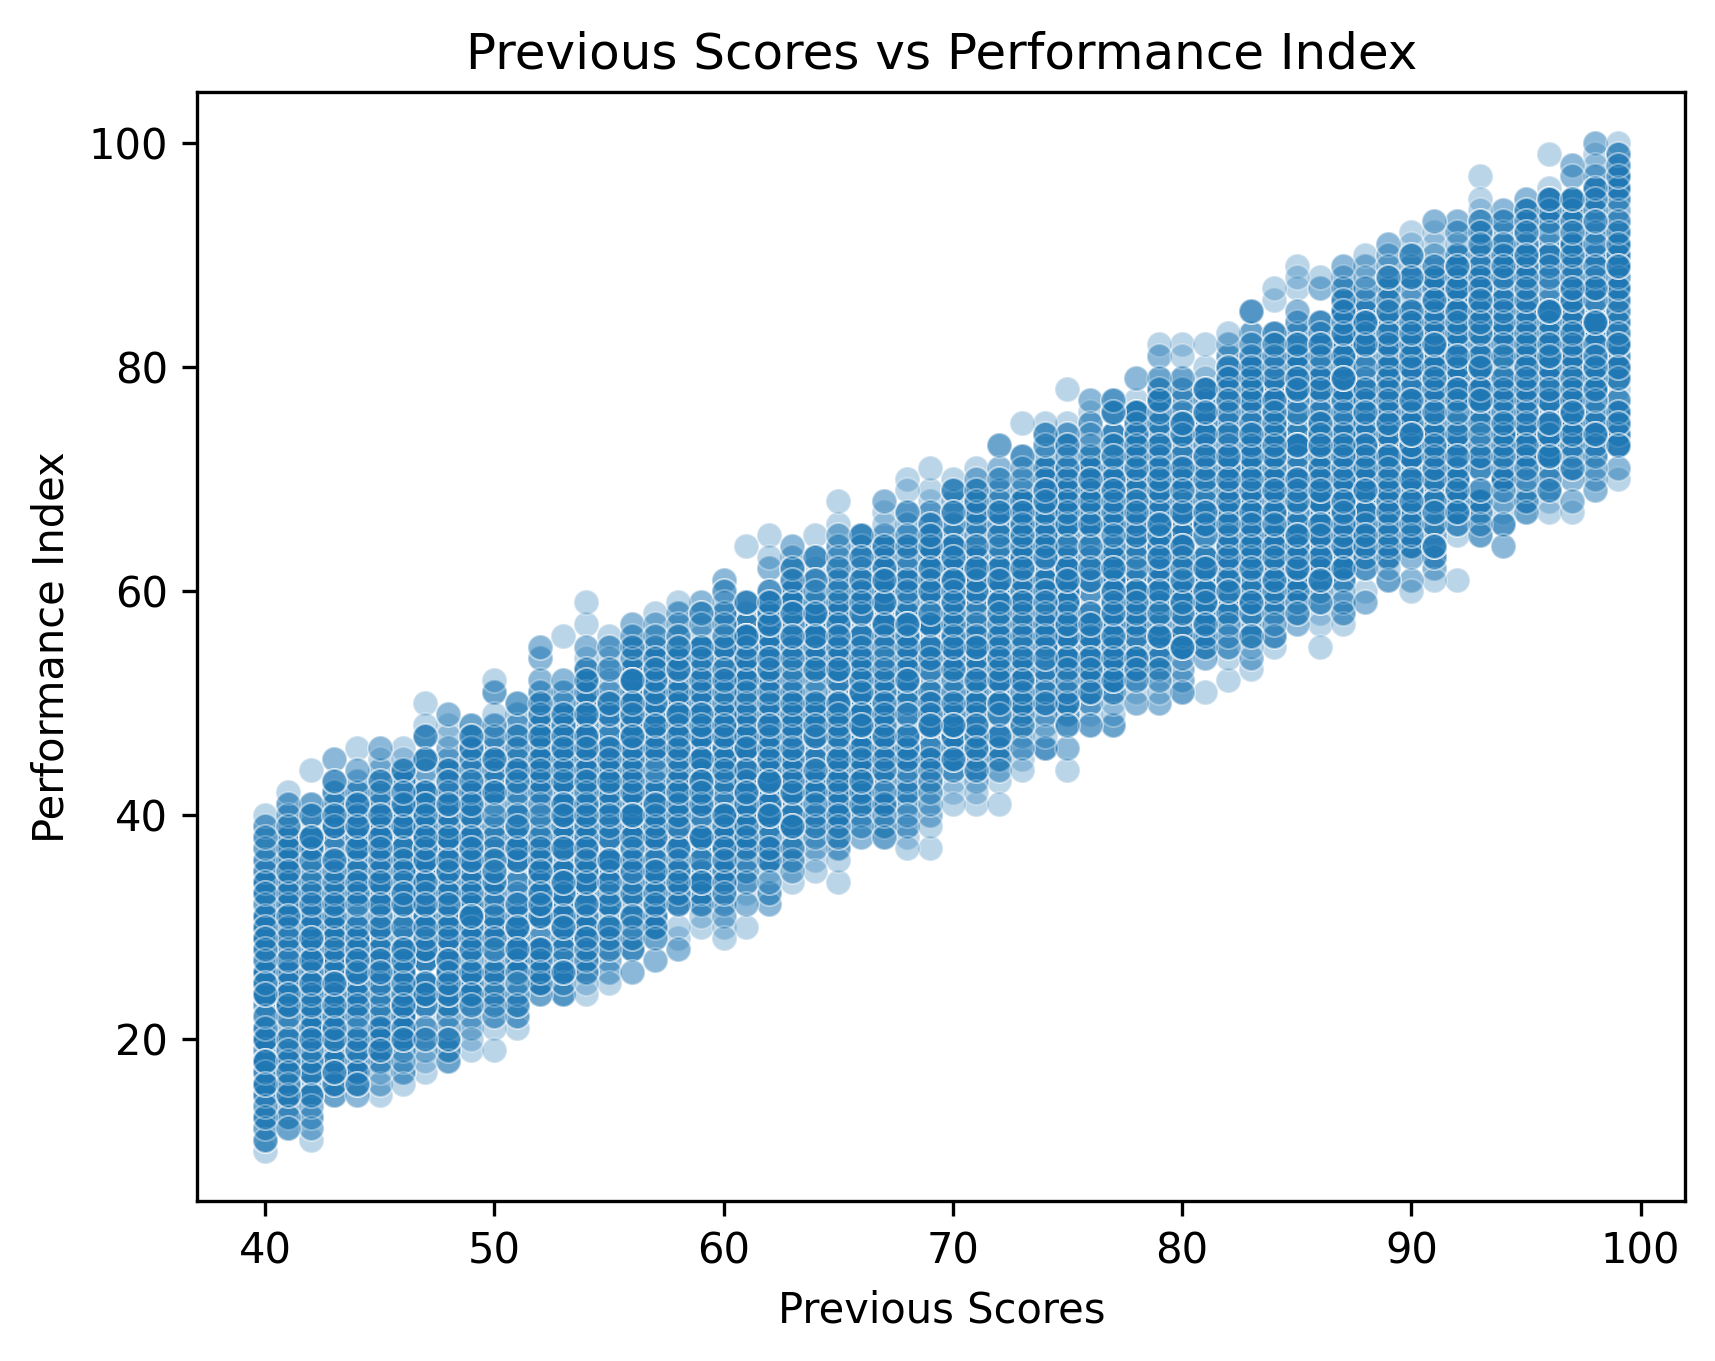
\includegraphics[width=0.44\textwidth]{previous_scores.png}
    \caption{Relación entre Previous Scores y Performance Index.}
\end{figure}

Este fue el diagrama de dispersión más revelador del análisis exploratorio. Esto debido a que se observó una tendencia positiva muy clara y cercana a una relación lineal entre \texttt{Previous Scores} y \texttt{Performance Index}. En otras palabras, los estudiantes con mejor rendimiento previo tienden también a mostrar un mejor rendimiento actual. Lo cual tiene sentido y es lo esperado.

La forma del gráfico respalda fuertemente la idea del uso de una regresión lineal, ya que justamente este tipo de modelo aprovecha relaciones posiblemente lineales entre variables predictoras y la variable objetivo.

\subsubsection{Extracurricular Activities vs Performance Index}

\begin{figure}[H]
    \centering
    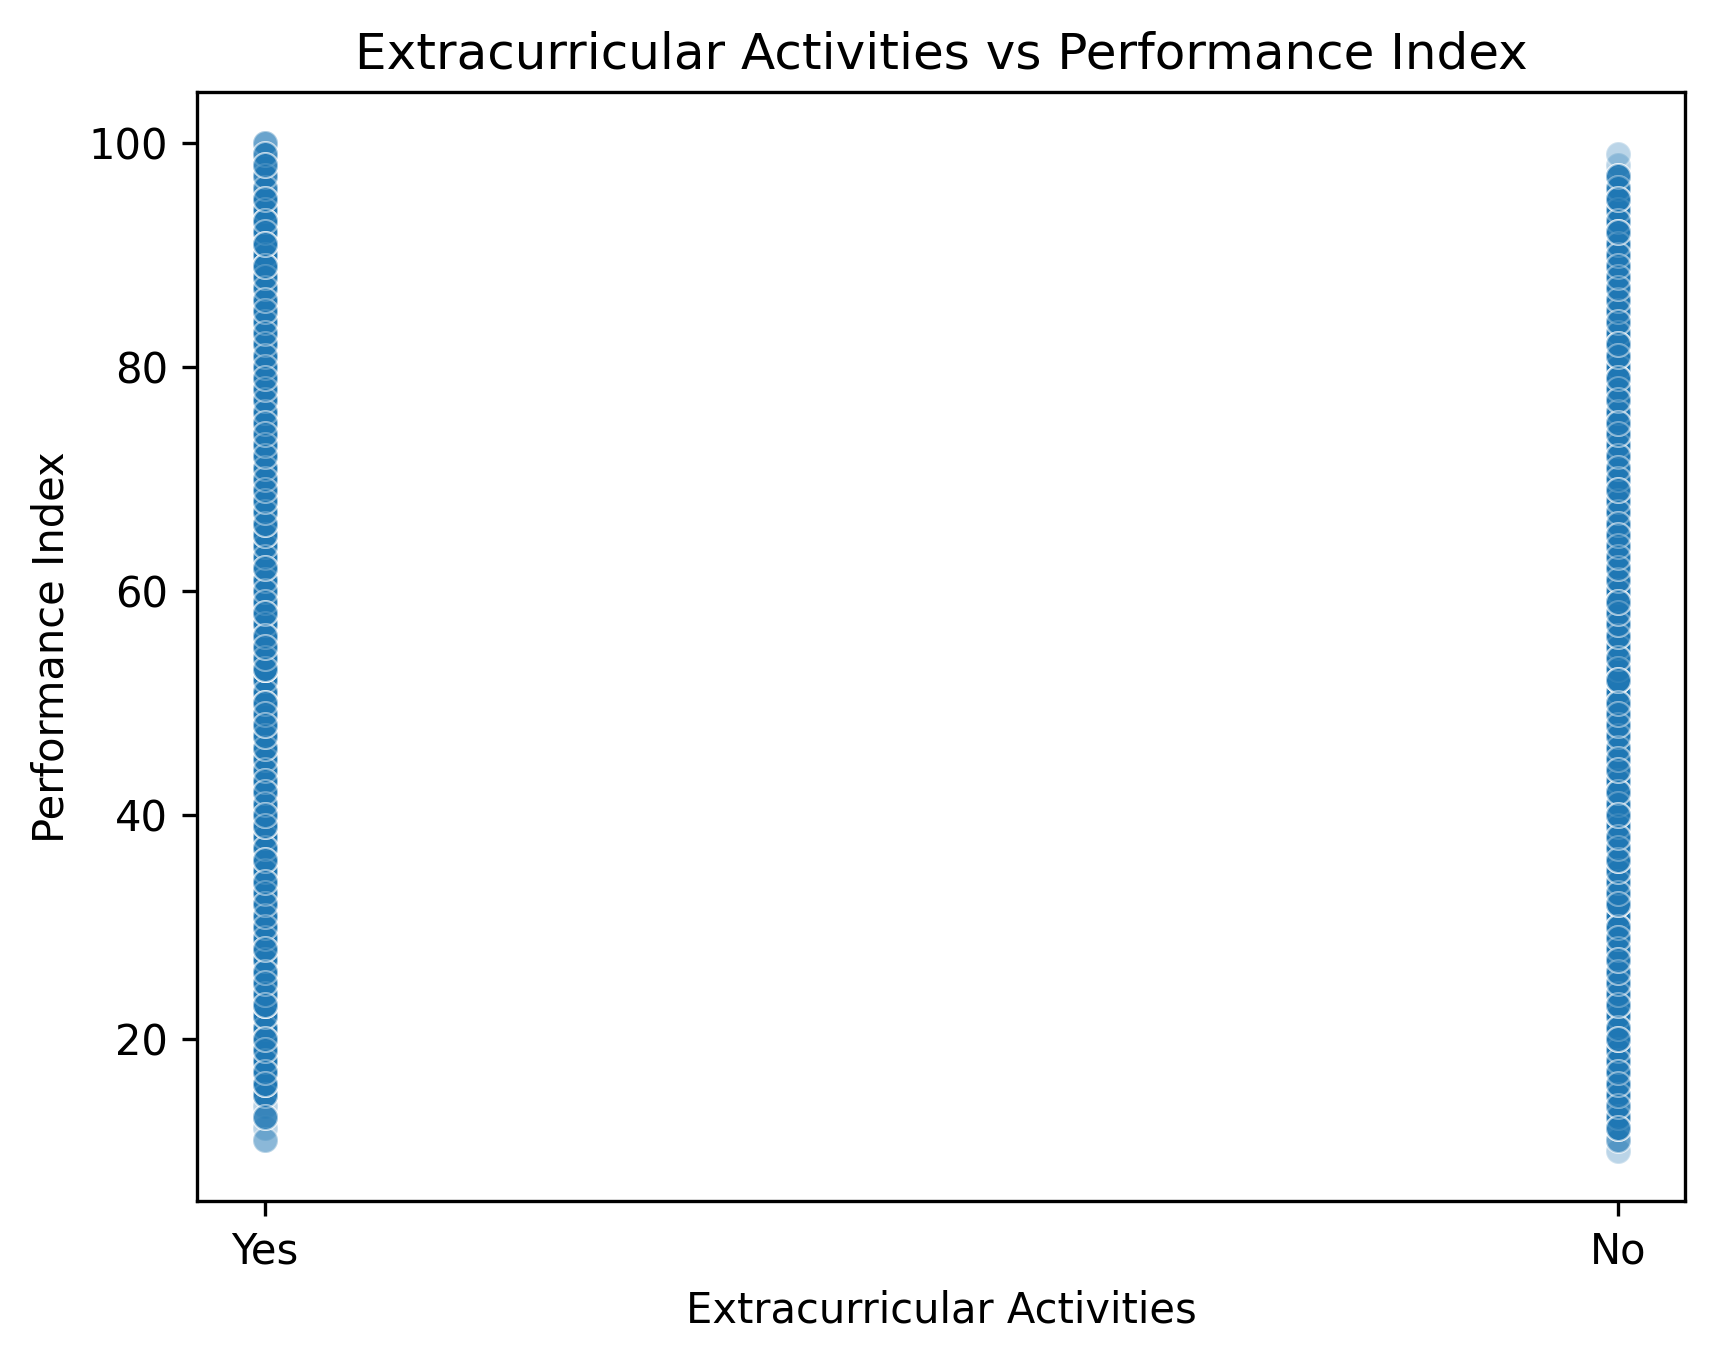
\includegraphics[width=0.44\textwidth]{extracurricular_activities.png}
    \caption{Relación entre Extracurricular Activities y Performance Index.}
\end{figure}

Al tratarse de una variable categórica binaria, el gráfico se redujo a dos columnas de puntos, una para \texttt{Yes} y otra para \texttt{No}. Visualmente no se observó una diferencia extremadamente marcada entre ambas categorías, lo que sugiere que esta variable no tiene una influencia tan fuerte como \texttt{Previous Scores} o \texttt{Hours Studied}.

\subsubsection{Sleep Hours vs Performance Index}

\begin{figure}[H]
    \centering
    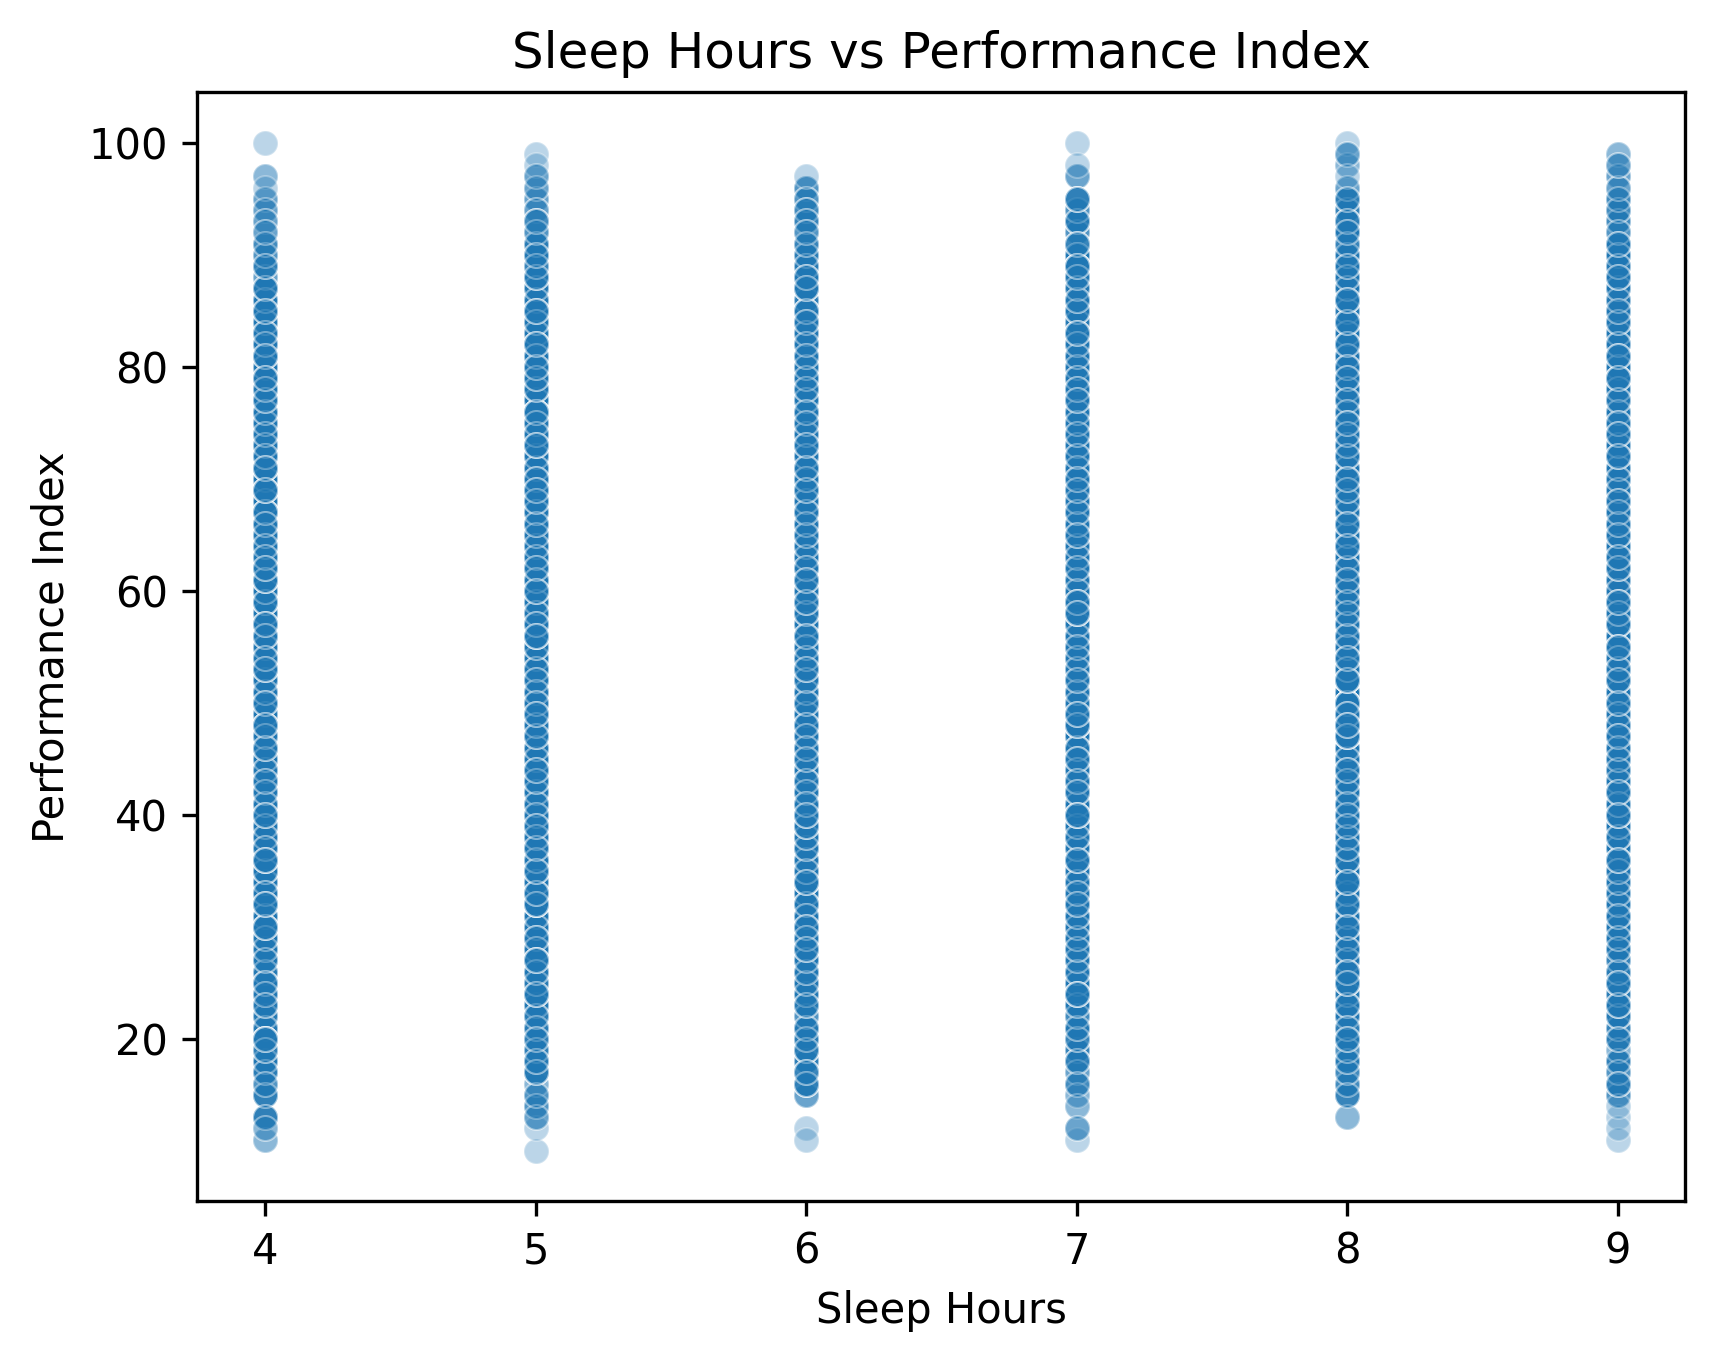
\includegraphics[width=0.44\textwidth]{sleep_hours.png}
    \caption{Relación entre Sleep Hours y Performance Index.}
\end{figure}

En el caso de \texttt{Sleep Hours}, la relación visual con el rendimiento fue bastante dispersa. Esto debido a que no se identificó una tendencia lineal fuerte ni ascendente o descendente. Este resultado da a entender que, las horas de sueño tienen una influencia limitada sobre el \texttt{Performance Index} según este dataset.

\subsubsection{Sample Question Papers Practiced vs Performance Index}

\begin{figure}[H]
    \centering
    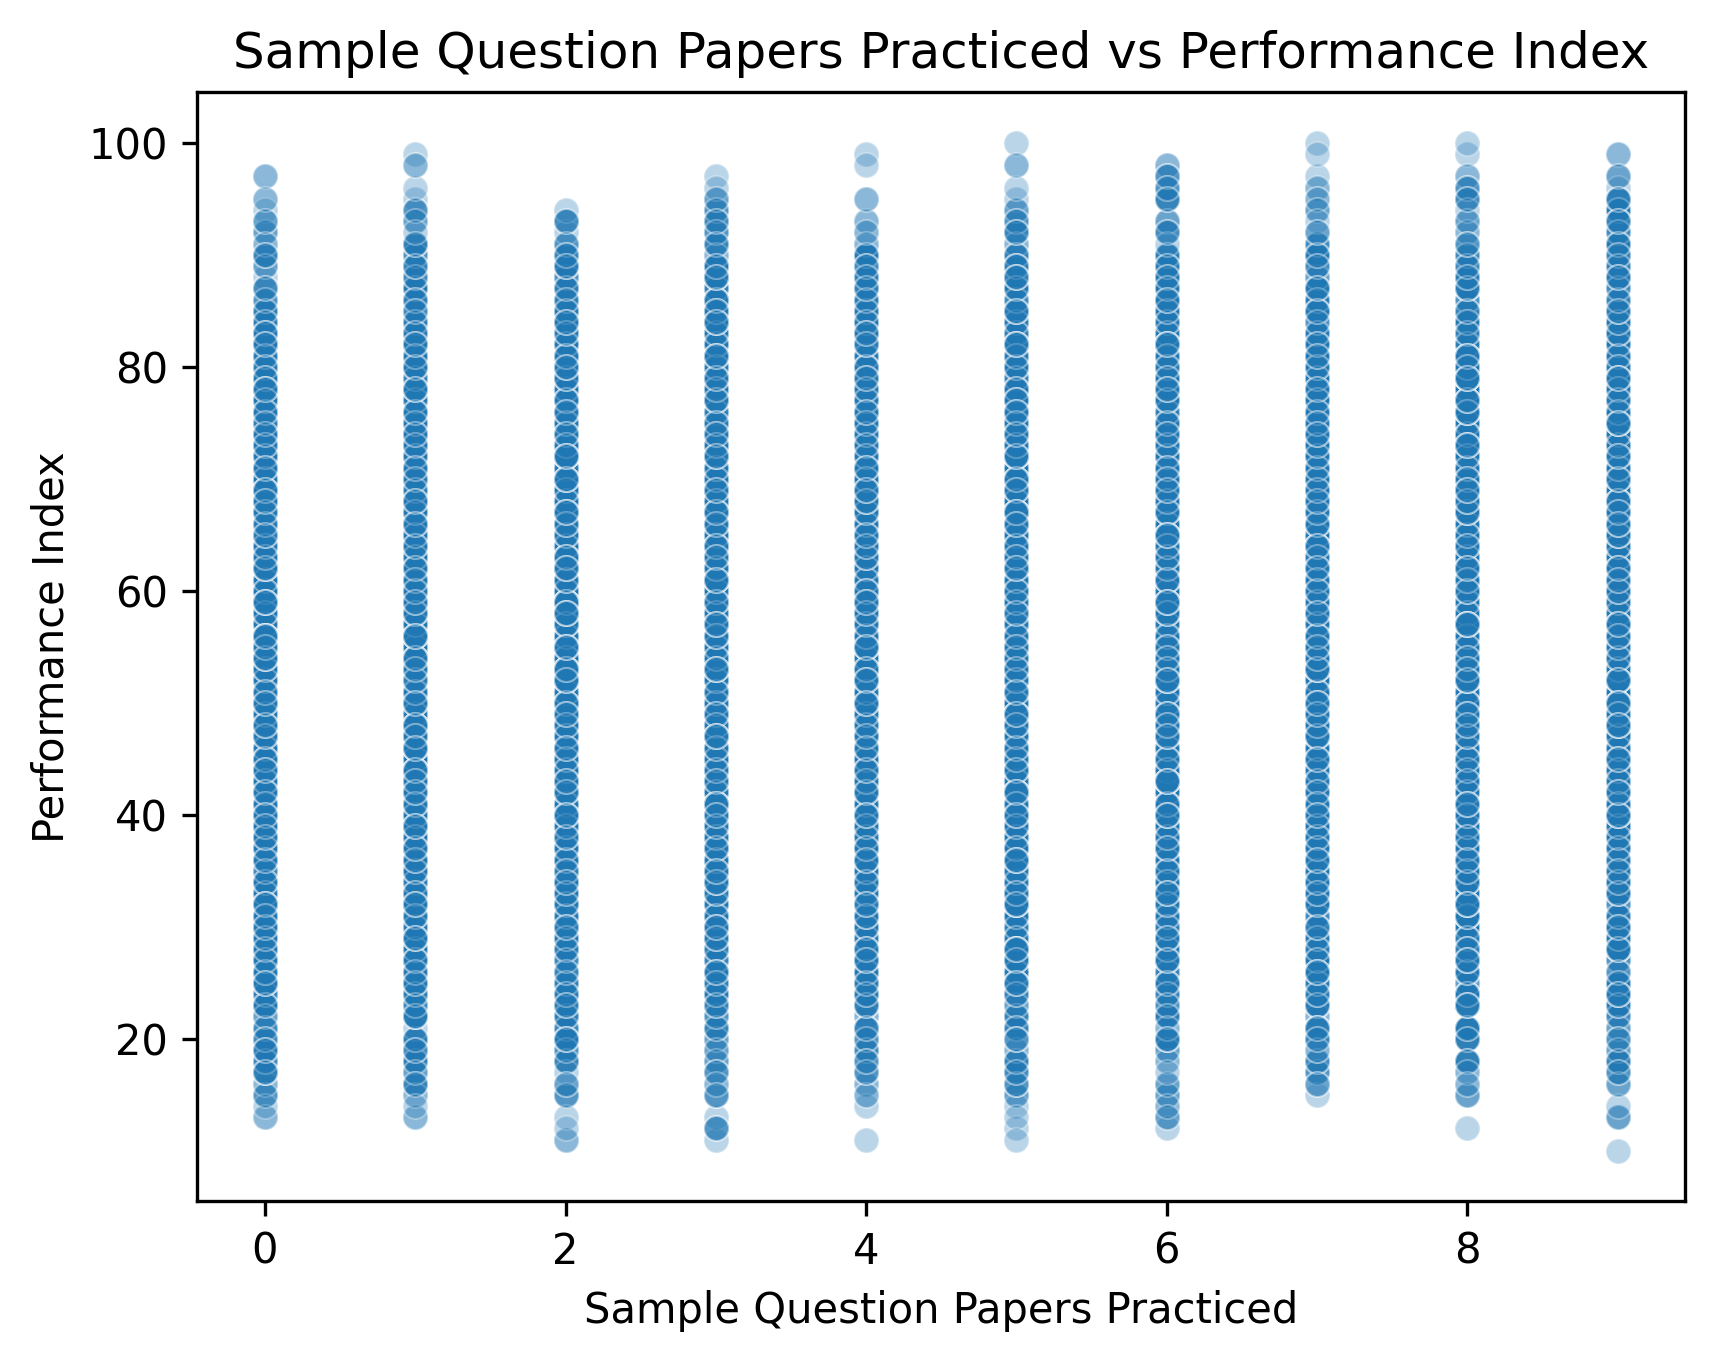
\includegraphics[width=0.44\textwidth]{sample_question_papers_practiced.png}
    \caption{Relación entre Sample Question Papers Practiced y Performance Index.}
\end{figure}

Este gráfico mostró una ligera tendencia positiva, aunque mucho más débil y dispersa que la observada en otras relaciones como \texttt{Previous Scores}. Podría interpretarse de la siguiente manera:  practicar más ejercicios ayuda al rendimiento, pero su efecto no es tan definitivo debido a que tiene bastante variabilidad.

Terminando el análisis de los diagramas de dispersión, estos permitieron identificar que \texttt{Previous Scores} y \texttt{Hours Studied} eran las variables con mayor capacidad de relación visual con la variable \texttt{Performance Index}. Esta última afirmación fue confirmada por la matriz de correlación.

\subsection{Matriz de correlación}

La matriz de correlación confirmó lo observado en los diagramas de dispersión. La variable \texttt{Previous Scores} presentó una correlación positiva muy fuerte con la variable \texttt{Performance Index}, mientras que \texttt{Hours Studied} mostró una correlación positiva moderada. Las demás variables tuvieron correlaciones bajas con la variable objetivo.

\begin{figure}[H]
    \centering
    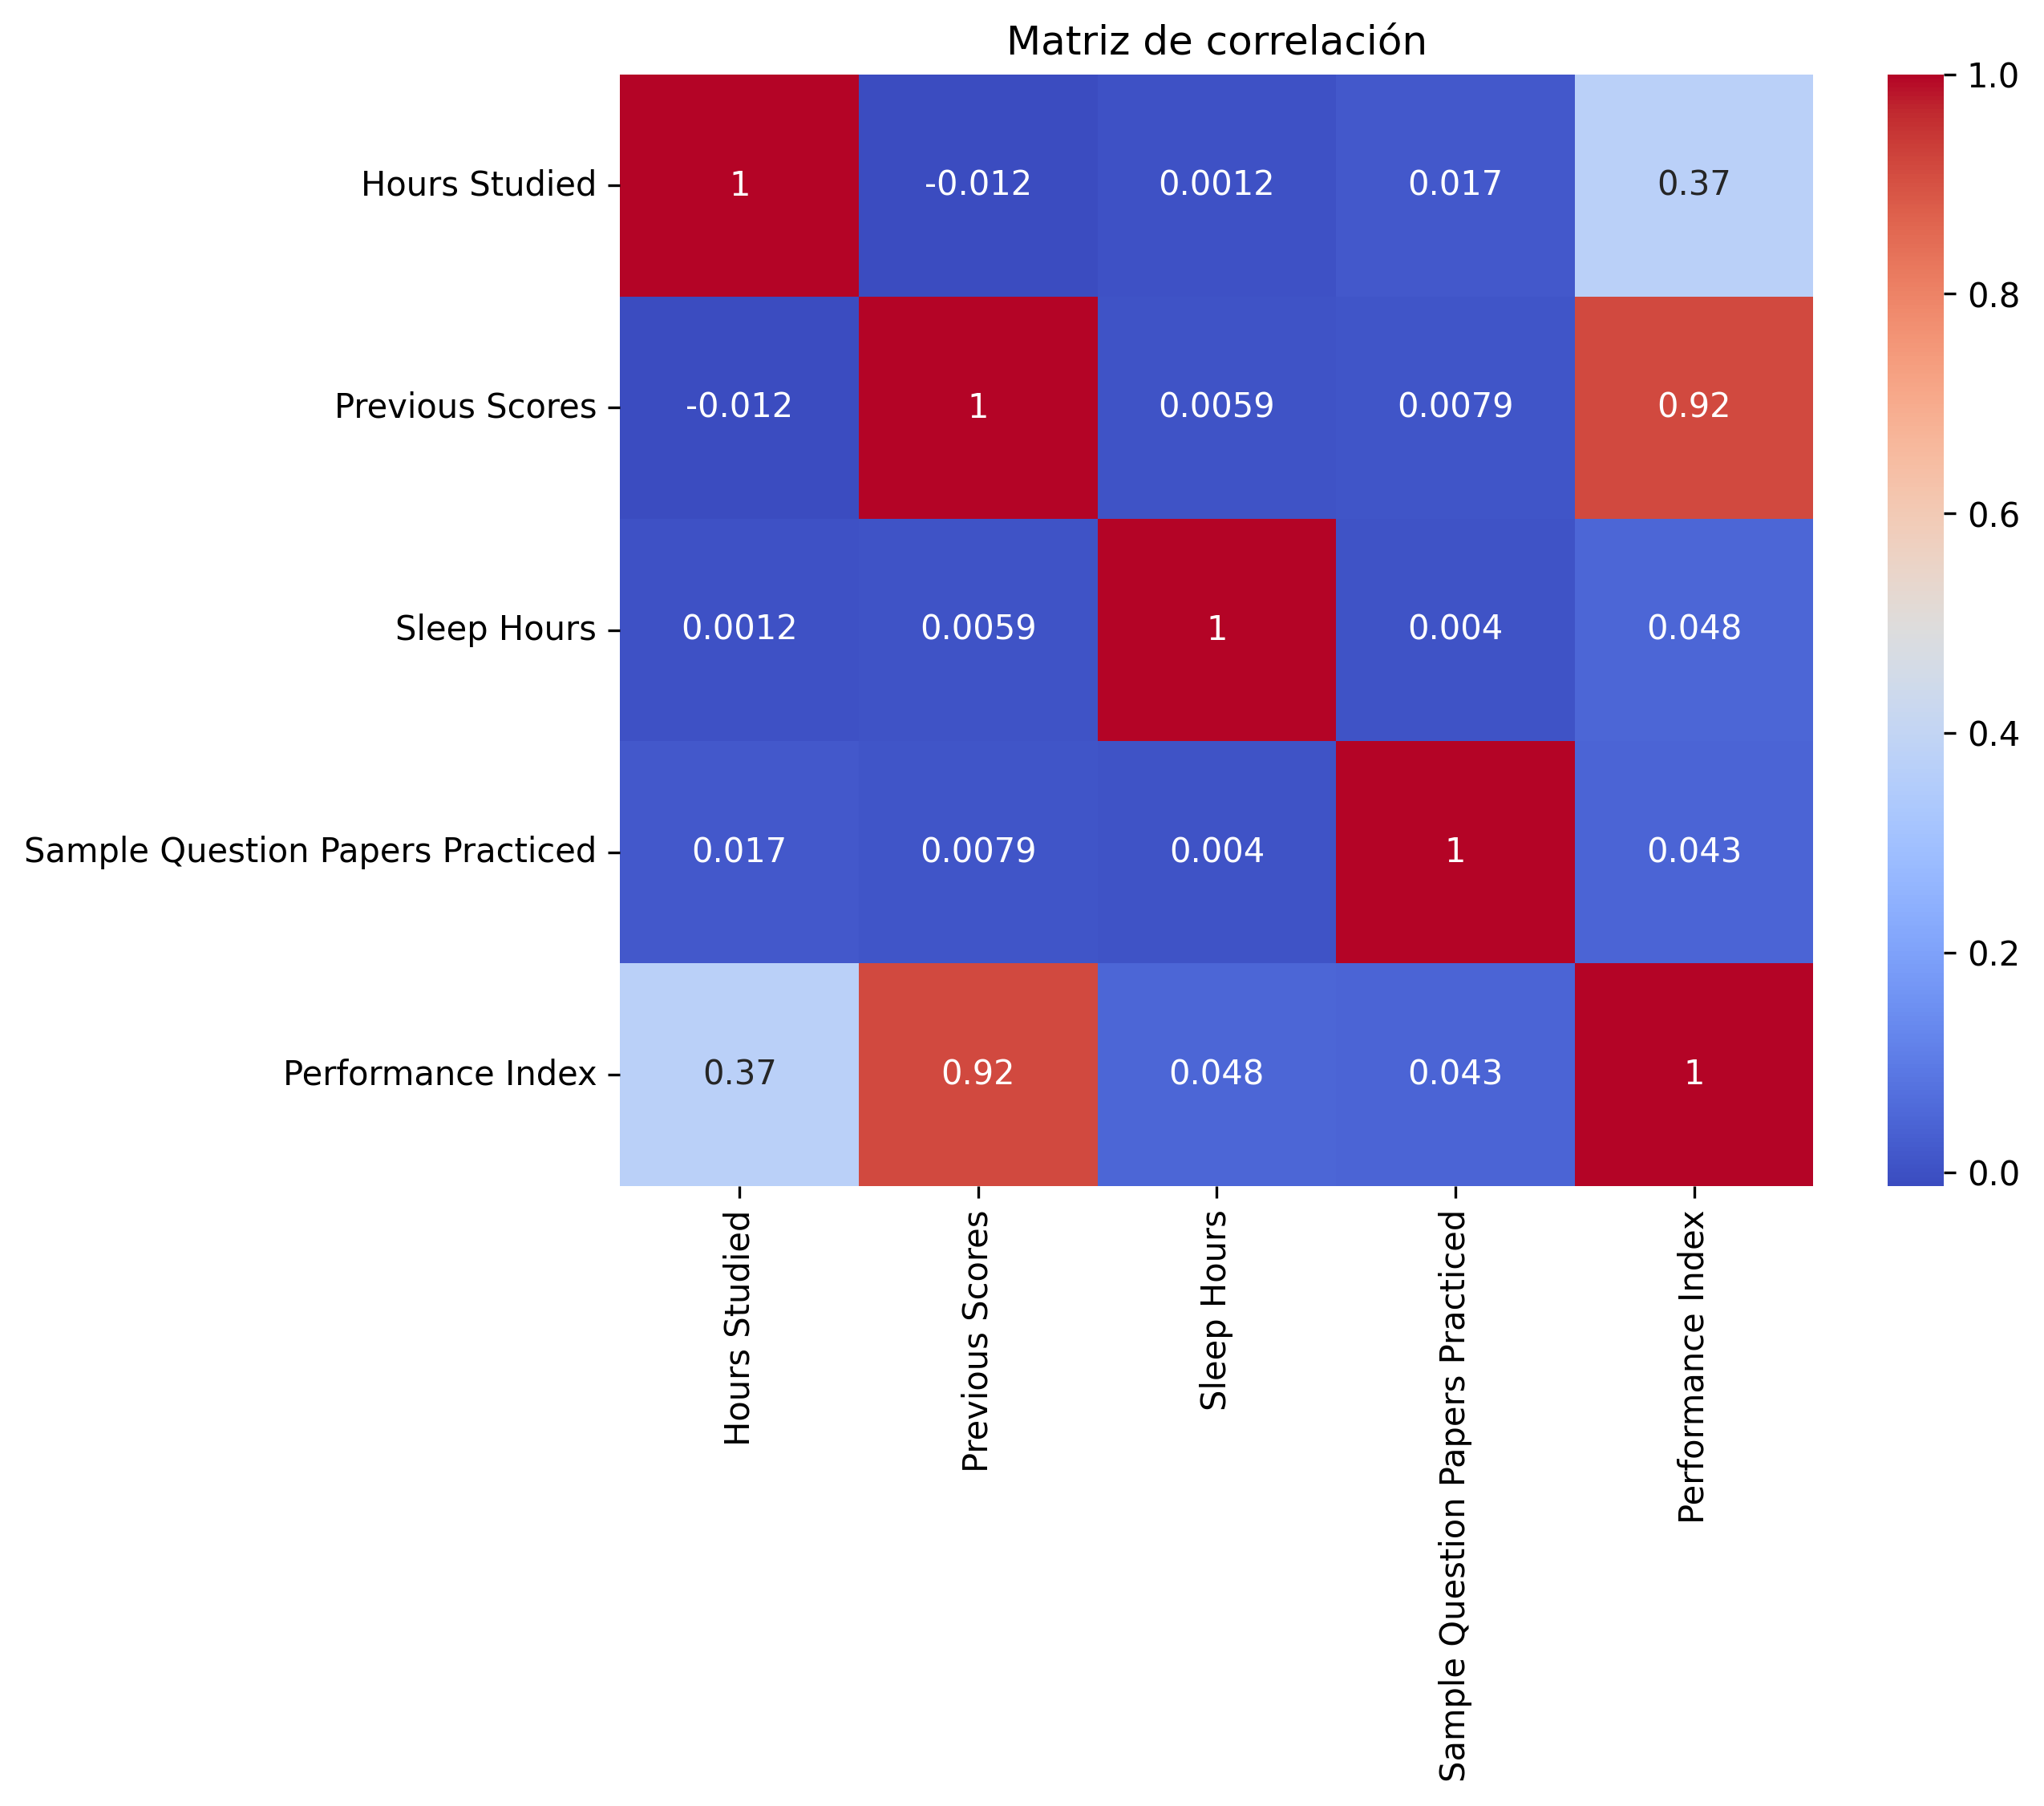
\includegraphics[width=0.46\textwidth]{heatmap_correlacion.png}
    \caption{Mapa de calor de la matriz de correlación.}
\end{figure}

El valor de correlación entre \texttt{Previous Scores} y \texttt{Performance Index} fue particularmente alto (un 0.92), lo cual refuerza la idea de que el desempeño previo es el predictor más importante dentro del dataset. \texttt{Hours Studied} presentó una correlación positiva moderada, aunque claramente menor (0.37). En cambio, \texttt{Sleep Hours} y \texttt{Sample Question Papers Practiced} mostraron valores muy cercanos a cero, lo que da a entender que es una relación lineal débil.

Otro aspecto importante que no se puede olvidar, es que las correlaciones entre las variables predictoras fueron bajas en general. Esto es realmente positivo, debido a que nos da a entender que el modelo si es candidato para la regresión lineal. Con esto se reduce problemas de multicolinealidad y facilita que cada variable aporte información sin redundancia excesiva.

La concordancia entre histogramas, boxplots, diagramas de dispersión y matriz de correlación permitió validar la consistencia del análisis realizado. En resumidas cuentas, las visualizaciones mostraron que el dataset era apropiado para aplicar un modelo de regresión lineal.

\section{División del dataset}

La división del dataset se realizó manualmente mediante muestreo aleatorio, sin utilizar \texttt{train\_test\_split}, como se mencionó en la especificación de la tarea. Se mezclaron primero los datos y luego se separaron en 70\% para entrenamiento, 15\% para validación y 15\% para prueba.

\CodeBlockSpaceBefore
\begin{lstlisting}[language=Python, caption={División manual del dataset}]
import numpy as np

df_shuffled = df.sample(frac=1, random_state=42).reset_index(drop=True)

n = len(df_shuffled)

train_end = int(0.7 * n)
val_end = int(0.85 * n)

train_df = df_shuffled[:train_end].copy()
val_df = df_shuffled[train_end:val_end].copy()
test_df = df_shuffled[val_end:].copy()

print("Train:", len(train_df))
print("Validation:", len(val_df))
print("Test:", len(test_df))
\end{lstlisting}
\CodeBlockSpaceAfter

Seguidamente se transformó la variable categórica \texttt{Extracurricular Activities} a valores numéricos para permitir su uso en el modelo matemático de regresión lineal.

\CodeBlockSpaceBefore
\begin{lstlisting}[language=Python, caption={Conversión de variable categórica y separación de X e y}]
train_df['Extracurricular Activities'] = train_df['Extracurricular Activities'].map({'Yes': 1, 'No': 0})
val_df['Extracurricular Activities'] = val_df['Extracurricular Activities'].map({'Yes': 1, 'No': 0})
test_df['Extracurricular Activities'] = test_df['Extracurricular Activities'].map({'Yes': 1, 'No': 0})

target = "Performance Index"

X_train = train_df.drop(target, axis=1).values
y_train = train_df[target].values

X_val = val_df.drop(target, axis=1).values
y_val = val_df[target].values

X_test = test_df.drop(target, axis=1).values
y_test = test_df[target].values
\end{lstlisting}
\CodeBlockSpaceAfter

\section{Preparación de datos para el modelo}

Antes de entrenar el modelo, se normalizaron las variables de entrada usando la media y desviación estándar del conjunto de entrenamiento. Esto fue importante porque las características tenían escalas distintas, y sin normalización el descenso del gradiente tendía a divergir considerablemente.

\CodeBlockSpaceBefore
\begin{lstlisting}[language=Python, caption={Normalización y agregado del bias}]
mean_train = X_train.mean(axis=0)
std_train = X_train.std(axis=0)

X_train = (X_train - mean_train) / std_train
X_val = (X_val - mean_train) / std_train
X_test = (X_test - mean_train) / std_train

X_train = np.c_[np.ones(X_train.shape[0]), X_train]
X_val = np.c_[np.ones(X_val.shape[0]), X_val]
X_test = np.c_[np.ones(X_test.shape[0]), X_test]
\end{lstlisting}
\CodeBlockSpaceAfter

El \textit{bias} corresponde al término independiente del modelo. Su inclusión permite que la recta o hiperplano de regresión no quede forzado a pasar por el origen, mejorando así la flexibilidad del ajuste.

\section{Implementación de la regresión lineal}

\subsection{Funciones auxiliares}

Se definieron dos funciones básicas: una para generar predicciones y otra para calcular el error cuadrático medio (MSE).

\CodeBlockSpaceBefore
\begin{lstlisting}[language=Python, caption={Funciones auxiliares del modelo}]
def predict(X, theta):
    return X @ theta

def mse(y_true, y_pred):
    return np.mean((y_true - y_pred) ** 2)
\end{lstlisting}
\CodeBlockSpaceAfter

\subsection{Experimento A: Batch Gradient Descent}

En Batch Gradient Descent, el gradiente se calcula utilizando la totalidad del conjunto de entrenamiento en cada época. Esto hace que el proceso sea más estable, aunque normalmente más costoso por iteración que otras variantes.

\CodeBlockSpaceBefore
\begin{lstlisting}[language=Python, caption={Implementación de Batch Gradient Descent}]
# X_train (variables de entrada de entrenamiento), Y_train (valores reales de entrenamiento)
# X_val (variables de validación), Y_val (valores reales de validación)
# Alpha (tasa de aprendizaje), Rep (Cantidad de repeticiones)
def batch_gradient_descent(X_train, y_train, X_val, y_val, alpha=0.01, rep=1000):
    # Matriz en 0
    m, n = X_train.shape
    theta = np.zeros(n)

    # Lista para guardar el MSE
    train_losses = []
    val_losses = []

    for epoch in range(rep):
        # Calcular predicciones
        y_pred = predict(X_train, theta)
        # Calcular error
        error = y_pred - y_train

        # Fórmula planteada (con la derivada de MSE)
        gradient = (2 / m) * (X_train.T @ error)
        theta = theta - alpha * gradient

        train_losses.append(mse(y_train, predict(X_train, theta)))
        val_losses.append(mse(y_val, predict(X_val, theta)))

    return theta, train_losses, val_losses
\end{lstlisting}
\CodeBlockSpaceAfter

El algoritmo sigue la regla general:

\[
\theta := \theta - \alpha \cdot \nabla L(\theta)
\]

donde \(\theta\) representa los parámetros del modelo, \(\alpha\) la tasa de aprendizaje y \(\nabla L(\theta)\) el gradiente de la función de costo.

\subsection{Entrenamiento y evaluación del experimento A}

\CodeBlockSpaceBefore
\begin{lstlisting}[language=Python, caption={Entrenamiento y evaluación de Batch Gradient Descent}]
theta_batch, train_loss_batch, val_loss_batch = batch_gradient_descent(
    X_train, y_train, X_val, y_val,
    alpha=0.01,
    rep=1000
)

y_test_pred_batch = predict(X_test, theta_batch)
test_mse_batch = mse(y_test, y_test_pred_batch)

print("MSE en test (Batch):", test_mse_batch)
\end{lstlisting}
\CodeBlockSpaceAfter

Con esta configuración se obtuvo un MSE aproximado de 4.08 en el conjunto de prueba. La curva de entrenamiento y validación mostró una convergencia estable, sin señales claras de sobreajuste.

\begin{figure}[H]
    \centering
    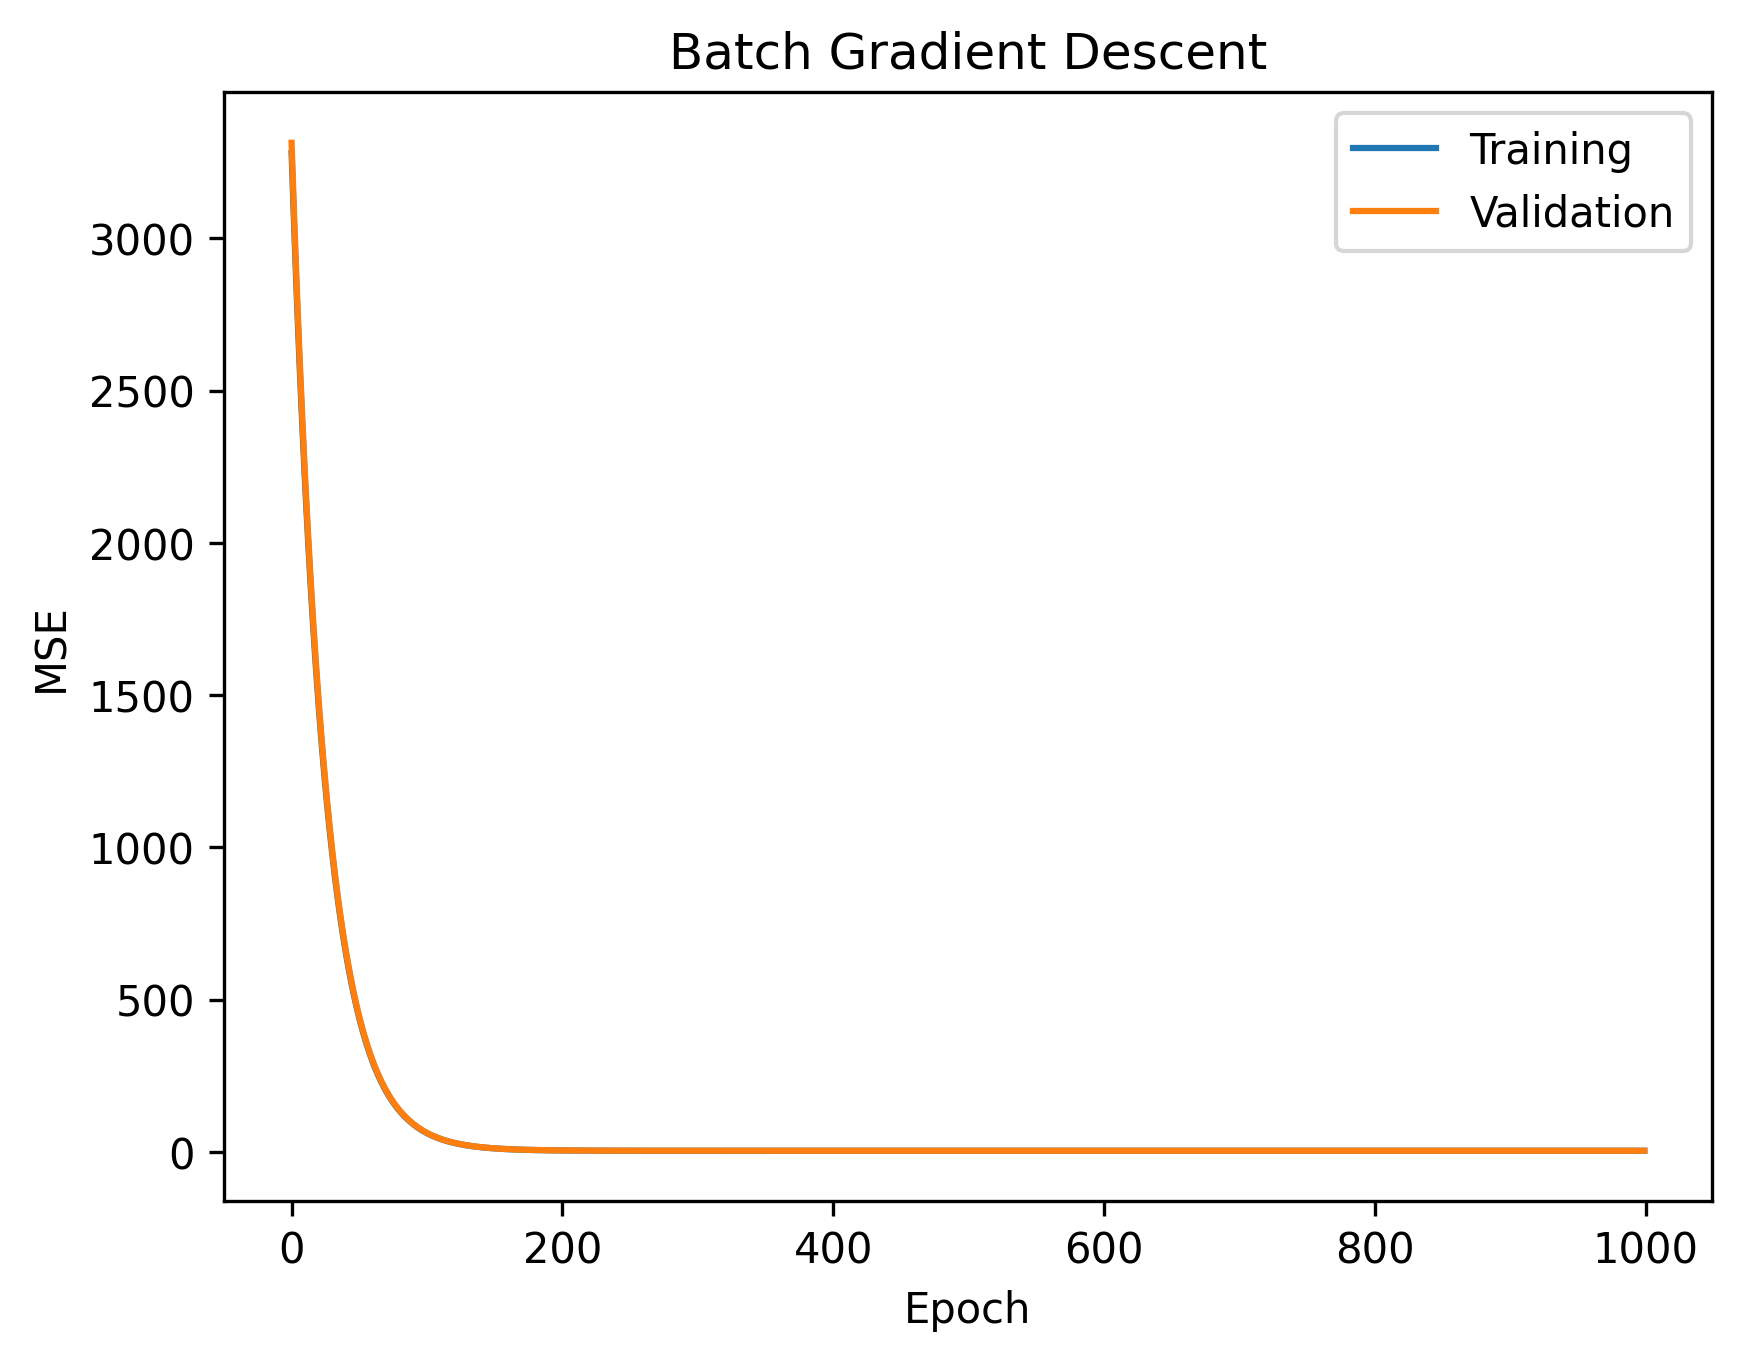
\includegraphics[width=0.46\textwidth]{loss_batch.png}
    \caption{Curvas de entrenamiento y validación para Batch Gradient Descent.}
\end{figure}

Durante las primeras épocas, el error disminuyó de manera pronunciada, lo cual indica que el modelo aprendió rápidamente una aproximación razonable de la relación entre las variables de entrada y la variable objetivo. Posteriormente, la curva comenzó a estabilizarse, mostrando una convergencia adecuada.

La cercanía entre las curvas de entrenamiento y validación indica que el modelo no estaba memorizando los datos de entrenamiento, sino generalizando bien hacia datos no vistos dentro del conjunto de validación. Esto fue una señal favorable de que la configuración de aprendizaje utilizada era apropiada.

\subsection{Experimento B: Mini-Batch Gradient Descent}

En Mini-Batch Gradient Descent, el gradiente no se calcula con todo el conjunto de entrenamiento a la vez, sino con pequeños subconjuntos llamados mini-batches. Esto permite realizar varias actualizaciones de parámetros dentro de una misma época y suele volver el entrenamiento más flexible.

\CodeBlockSpaceBefore
\begin{lstlisting}[language=Python, caption={Implementación de Mini-Batch Gradient Descent}]
# X_train (variables de entrada de entrenamiento), Y_train (valores reales de entrenamiento)
# X_val (variables de validación), Y_val (valores reales de validación)
# Alpha (tasa de aprendizaje), Rep (Cantidad de repeticiones), Batch_size (tamaño de cada mini-batch)
def mini_batch_gradient_descent(X_train, y_train, X_val, y_val, alpha=0.01, rep=1000, batch_size=32):
    # Matriz en 0
    m, n = X_train.shape
    theta = np.zeros(n)

    # Lista para guardar el MSE
    train_losses = []
    val_losses = []

    for epoch in range(rep):
        # Mezclar datos aleatoriamente en cada repetición
        indices = np.random.permutation(m)
        X_shuffled = X_train[indices]
        y_shuffled = y_train[indices]

        # Recorrer pequeños grupos de datos
        for i in range(0, m, batch_size):
            X_batch = X_shuffled[i:i+batch_size]
            y_batch = y_shuffled[i:i+batch_size]

            # Calcular predicciones del mini-batch
            y_pred_batch = predict(X_batch, theta)
            # Calcular error del mini-batch
            error_batch = y_pred_batch - y_batch

            # Fórmula planteada (con la derivada de MSE)
            gradient = (2 / len(y_batch)) * (X_batch.T @ error_batch)
            theta = theta - alpha * gradient

        train_losses.append(mse(y_train, predict(X_train, theta)))
        val_losses.append(mse(y_val, predict(X_val, theta)))

    return theta, train_losses, val_losses
\end{lstlisting}
\CodeBlockSpaceAfter

\subsection{Entrenamiento y evaluación del experimento B}

\CodeBlockSpaceBefore
\begin{lstlisting}[language=Python, caption={Entrenamiento y evaluación de Mini-Batch Gradient Descent}]
theta_mini, train_loss_mini, val_loss_mini = mini_batch_gradient_descent(
    X_train, y_train, X_val, y_val,
    alpha=0.01,
    rep=1000,
    batch_size=32
)

y_test_pred_mini = predict(X_test, theta_mini)
test_mse_mini = mse(y_test, y_test_pred_mini)

print("MSE en test (Mini-Batch):", test_mse_mini)
\end{lstlisting}
\CodeBlockSpaceAfter

El experimento B obtuvo un MSE aproximado de 4.09 en el conjunto de prueba. Este valor fue muy cercano al obtenido con Batch Gradient Descent, aunque la curva de validación mostró pequeñas oscilaciones, comportamiento esperable al utilizar subconjuntos de datos en las actualizaciones.

\begin{figure}[H]
    \centering
    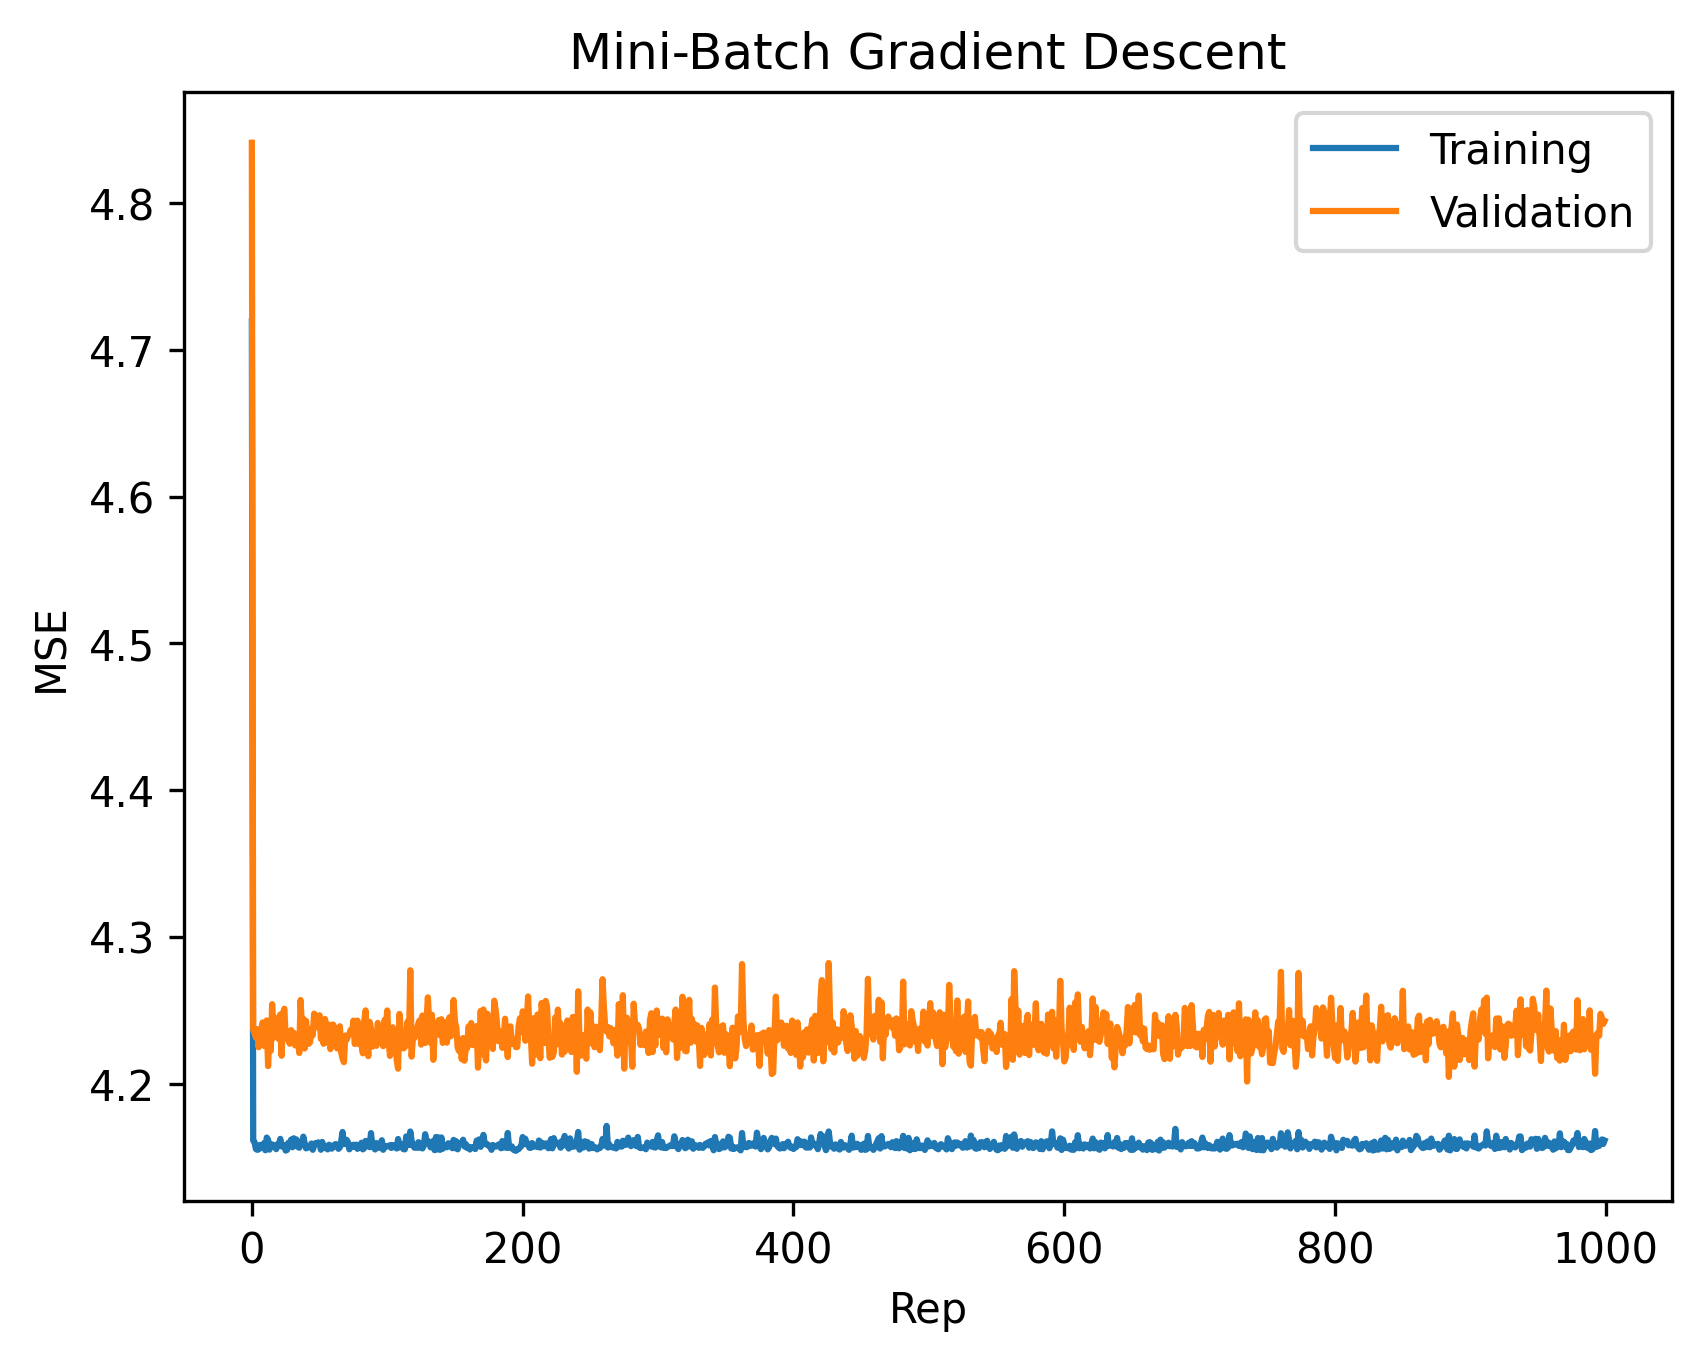
\includegraphics[width=0.46\textwidth]{loss_minibatch.png}
    \caption{Curvas de entrenamiento y validación para Mini-Batch Gradient Descent.}
\end{figure}

A diferencia de Batch Gradient Descent, aquí el error de validación presenta ligeras variaciones a lo largo del entrenamiento. Esto no necesariamente es una señal negativa, sino una consecuencia natural de que el gradiente se estima con pequeños grupos de datos y no con la totalidad del conjunto de entrenamiento.

Aun con esas pequeñas oscilaciones, el modelo mantuvo un comportamiento estable y logró un desempeño muy cercano al de Batch Gradient Descent. Esto sugiere que ambas variantes son adecuadas para este problema, aunque Batch mostró una ventaja mínima en el conjunto de prueba.

\section{Evaluación del modelo}

La métrica principal utilizada fue el error cuadrático medio (MSE). Esta métrica se calculó manualmente y se registró durante las épocas de entrenamiento para los conjuntos de entrenamiento y validación.

En ambos experimentos, las curvas mostraron convergencia adecuada. En el caso de Batch Gradient Descent, el entrenamiento fue particularmente estable y terminó con un MSE de prueba ligeramente menor. En Mini-Batch Gradient Descent, aunque hubo pequeñas fluctuaciones, el resultado final fue también bastante bueno.

Si se toma la raíz cuadrada del MSE, el error promedio en términos del índice de rendimiento es bastante bajo, lo cual indica que el modelo logra aproximar correctamente la variable objetivo. Considerando que \texttt{Performance Index} toma valores en un rango amplio, los errores obtenidos pueden considerarse satisfactorios.

\section{Análisis de resultados}

Los resultados obtenidos indican que ambos algoritmos fueron efectivos para modelar la relación entre las variables predictoras y el índice de rendimiento. Batch Gradient Descent obtuvo un MSE de prueba levemente inferior al de Mini-Batch Gradient Descent, lo que sugiere un ajuste ligeramente mejor bajo la configuración utilizada.

La diferencia entre ambos métodos fue pequeña, por lo que en este dataset ambos pueden considerarse adecuados. No se observaron evidencias claras de overfitting, ya que las curvas de entrenamiento y validación se mantuvieron cercanas a lo largo del proceso.

También es importante resaltar que los resultados del modelado son coherentes con el análisis exploratorio previo. Las variables que visualmente parecían más relacionadas con \texttt{Performance Index}, especialmente \texttt{Previous Scores} y en menor medida \texttt{Hours Studied}, fueron precisamente las que permitieron al modelo alcanzar un error bajo. Esto refuerza la idea de que el EDA no fue solo una etapa descriptiva, sino una base importante para justificar el comportamiento posterior de la regresión lineal.

\begin{table}[H]
\centering
\caption{Comparación inicial entre los dos experimentos principales}
\begin{tabular}{@{}lccc@{}}
\toprule
Método & Alpha & Repeticiones & MSE Test \\ \midrule
Batch Gradient Descent & 0.01 & 1000 & 4.0753 \\
Mini-Batch Gradient Descent & 0.01 & 1000 & 4.0913 \\ \bottomrule
\end{tabular}
\end{table}

A partir de esta comparación puede decirse que Batch Gradient Descent ofreció el mejor resultado final, aunque por una diferencia muy pequeña. En un contexto práctico, ambos métodos tendrían un desempeño bastante parecido sobre este conjunto de datos.


En el caso de realizar las 10 ejecuciones con diferentes hiperparámetros, se pudo observar que existe una relación entre el valor de alpha y la cantidad de épocas necesarias para alcanzar un MSE bajo. En general, la tasa de aprendizaje y la cantidad de épocas afectan la convergencia de los dos métodos.
\begin{table}[H]
\caption{Resultados de las 10 ejecuciones con diferentes hiperparámetros}
\label{tab:comparativa_gd}
\centering
\resizebox{\columnwidth}{!}{
\begin{tabular}{@{}ccccc@{}}
\toprule
\textbf{Alpha ($\alpha$)} & \textbf{Epochs} & \textbf{B. Size} & \textbf{MSE Batch} & \textbf{MSE M-Batch} \\ \midrule
0.001 & 500  & 16 & 465.7088 & 4.0758 \\
0.001 & 1000 & 32 & 67.0938  & 4.0765 \\
0.001 & 2000 & 64 & 5.3395   & 4.0758 \\ \addlinespace
0.01  & 500  & 16 & 4.0756   & 4.0922 \\
0.01  & 1000 & 32 & 4.0753   & 4.0841 \\
0.01  & 2000 & 64 & 4.0753   & 4.0756 \\ \addlinespace
0.1   & 500  & 16 & 4.0753   & 4.4675 \\
0.1   & 1000 & 32 & 4.0753   & 4.1666 \\
0.1   & 2000 & 32 & 4.0753   & 4.0998 \\ \addlinespace
0.2   & 400  & 64 & 4.0753   & 4.1468 \\ \bottomrule
\end{tabular}%
}
\end{table}

Al observar la tabla, lo primero que salta a la vista es que el Batch Gradient Descent es muy lento cuando la tasa de aprendizaje ($\alpha$) es pequeño. Con $\alpha = 0.001$ y 500 épocas, el error es muy alto ($465.70$), y solo empieza a dar buenos resultados cuando se sube a 2000 épocas. En cambio, el Mini-Batch desde el principio ya logra un error bajo de $4.07$, sin importar cuántas épocas se utilicen. Esto pasa porque el Mini-Batch hace muchos ajustes por cada época, mientras que el Batch solo hace uno. Sin embargo, cuando se usa un $\alpha$ más alto ($0.1$ o $0.2$), el Batch se vuelve más preciso, mientras que el Mini-Batch empieza a "rebotar" un poco y su error sube a $4.46$ o $4.14$. Esto indica que el Mini-Batch es ideal para llegar rápido a una buena solución, pero el Batch es mejor para quedarse clavado en el punto exacto cuando el paso de aprendizaje es el adecuado.

\begin{figure}[H]
    \centering
    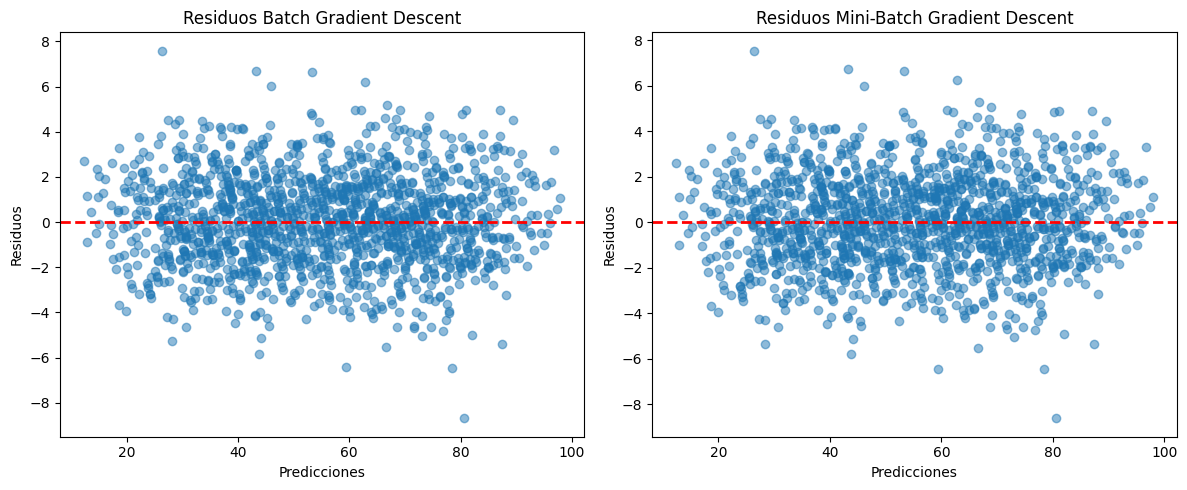
\includegraphics[width=0.46\textwidth]{residuo_vs_prediccion.png}
    \caption{Gráfico de residuos vs predicción para el mejor modelo entrenado.}
\end{figure}

Al comparar las gráficas de Batch y Mini-Batch Gradient Descent, se observa que ambos algoritmos llegan a una solución prácticamente idéntica, lo que valida que ambos convergieron al mismo modelo óptimo. Los puntos se distribuyen de forma aleatoria y uniforme alrededor de la línea horizontal en cero, lo cual es una excelente señal: significa que el modelo es adecuado y que los errores meramente ruidos. No se percibe un patrón de "embudo" ni tendencias curvas, lo que confirma que la relación encontrada es lineal. Aunque existen algunos valores atípicos (outliers) con residuos cercanos a $-8$ o $8$, la mayoría de las predicciones se mantienen en un margen de error aceptable, demostrando que el modelo predice con la misma eficacia tanto para notas bajas como para notas altas.

\section{Conclusiones}

A partir del análisis exploratorio se determinó que el dataset presentaba una estructura consistente, sin valores atípicos significativos y con relaciones lineales claras entre algunas variables y la variable objetivo. En particular, \texttt{Previous Scores} fue la variable con mayor correlación respecto al \texttt{Performance Index}, seguida por \texttt{Hours Studied}, mientras que las demás variables aportaron una influencia más débil.

La implementación manual de la regresión lineal permitió comprender de manera más profunda el funcionamiento del descenso del gradiente y la influencia de aspectos como la normalización de datos, el bias y la tasa de aprendizaje. Inicialmente, el modelo presentó problemas de divergencia, pero una vez normalizadas las variables la convergencia fue correcta. Esto dejó en evidencia que la preparación de los datos no es una etapa secundaria, sino una parte central del desempeño del algoritmo.

Finalmente, tanto Batch Gradient Descent como Mini-Batch Gradient Descent ofrecieron resultados satisfactorios. Batch obtuvo el mejor desempeño con un MSE ligeramente menor, aunque la diferencia con Mini-Batch fue reducida. En general, ambos modelos fueron capaces de predecir adecuadamente el rendimiento académico dentro del conjunto de prueba, y sus resultados mantuvieron coherencia con lo observado previamente en el análisis exploratorio.



\section*{Nota importante sobre figuras y cierre del trabajo}

Para compilar correctamente este documento, es necesario que las figuras utilizadas estén en la misma carpeta del archivo \texttt{.tex}. En este caso, los nombres empleados fueron los siguientes:

\begin{itemize}
    \item \texttt{histogramas.png}
    \item \texttt{boxplots.png}
    \item \texttt{hours\_studied.png}
    \item \texttt{previous\_scores.png}
    \item \texttt{extracurricular\_activities.png}
    \item \texttt{sleep\_hours.png}
    \item \texttt{sample\_question\_papers\_practiced.png}
    \item \texttt{heatmap\_correlacion.png}
    \item \texttt{loss\_batch.png}
    \item \texttt{loss\_minibatch.png}
    \item \texttt{residuo\_vs\_prediccion.png}
\end{itemize}

\end{document}